\chapter{MoVeIT KC705 firmware extensions}
\section{Introduction}
\noindent As explained in the previous chapters a good VHDL design, in order to improve readability, uses separate modules for each main task of the firmware. Each module is connected with wires (signals) to the others. The first half of this chapter will analyze the structure of the firmware used for the readout of the output of the ABACUS2 chip (section \ref{chip}), from now on named "KC705\_tera10 firmware", while the second half will be focused on my personal contribution to the project; this comprehends the HDL additions to the firmware and the simulations carried out with the Xilinx Vivado Software.
In this chapter there are also considerations on the implemented design and a short analysis of the most important post-implementation reports.
\newline
(\textit{tera10} in the firmware name comes from the TERA foundation, that is a scientific research foundation, recognized by the ministry of health, which since 1992 has been proposing the implementation of hadron therapy centers for the treatment of cancer through the applications of physics and advanced technologies in Italy and around the world.)
\begin{figure}[H]
	\centering
	
\includegraphics[width=0.2\linewidth]{IMG/ch4/TERA}
\end{figure}
\section{Firmware structure}\label{structure}
\noindent The starting point of the thesis work is a firmware developed by Richard Wheadon of INFN, Turin, designed to count the number of output logical pulses from the ABACUS2 chip, and store the corresponding count values on internal registers accessible from remote. This firmware has a hierarchical structure, shown in figure \ref{fig:tera10}, in which the main modules are:
\begin{figure}[H]
	\centering
	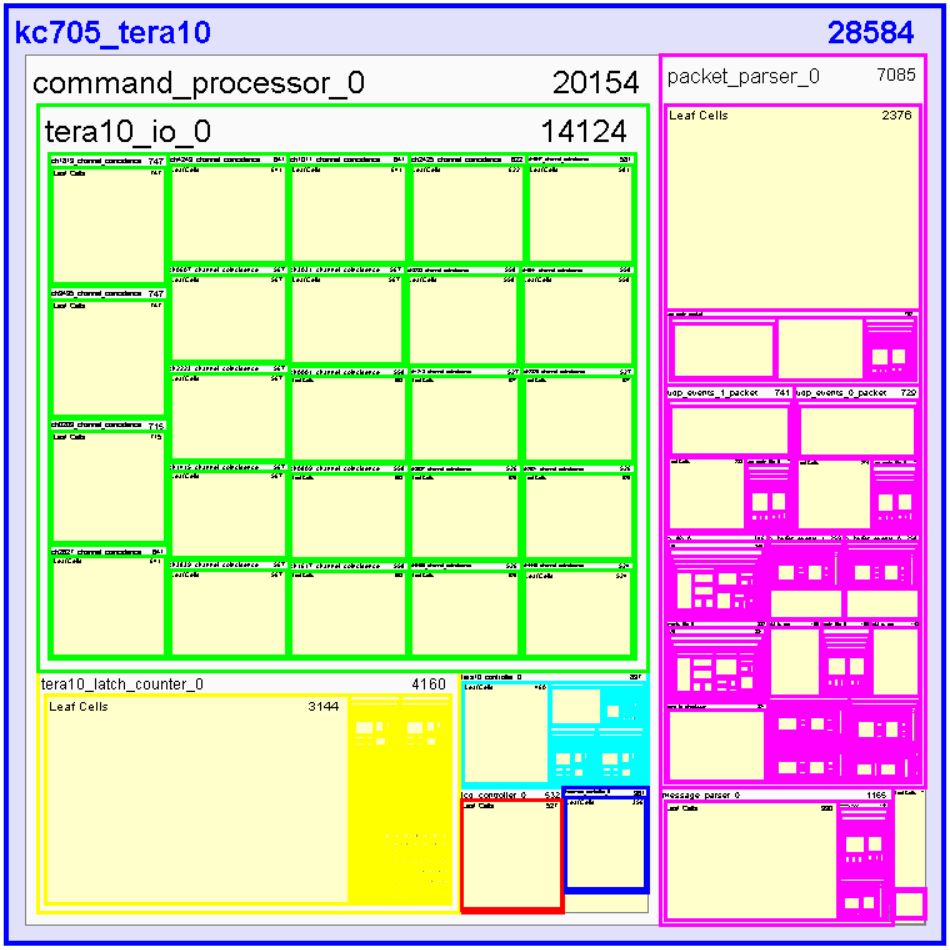
\includegraphics[width=0.75\linewidth]{IMG/ch4/HIERARCHY5}
	\caption{KC705\_tera10 firmware structure. GbPhy= purple; tera10\_latch\_counter= yellow; tera10\_io= green; tera10\_controller= light blue; lcd\_controller= red; hardware\_controller= blue; command\_processor= grey.}
	\label{fig:tera10}
\end{figure}
\begin{itemize}
	\item \textbf{KC705 TERA10}: this is the main module, it contains no logic, only component declarations and port-maps. In this module the firmware version ("B20C" for example) that will the displayed on the LCD can be set.
	%%%%%%%%%%%%%%%%%%%%%%%%%%%%%%%%%%%%%%%%%%%%%%%%%%%%%%%%%%%%%%%%%%%%%%%%%%
	\item \textbf{GbPhy}: the communication between FPGA and computer is done via Ethernet cable using a UDP (User Datagram Protocol) protocol. This is performed via firmware and also thanks to a dedicated chip connected on the board to the RJ45 connector called "PHY".
	\newline
	PHY is an abbreviation for "physical layer" and is an electronic component, usually implemented as an integrated circuit, mandatory to implement links between physical mediums such as copper or optical fiber. It basically converts data between a "clean" clocked digital stream form that is suitable only for very short distance communication (centimetres) and an analog form that is suitable for long range transmission (meters or more).
	The chip on the KC705 board is able to transmit data up to 1Gb/s.
	\newline
	The PHY is thus firmware controlled, in particular in the MoVeIT project the reception and sending of messages is managed by another project of the Turin INFN group called GbPhy. This thesis will  not focus on how it works, but only on its main characteristics~\cite{gbphy}.     
	\begin{figure}[H]
		\centering
		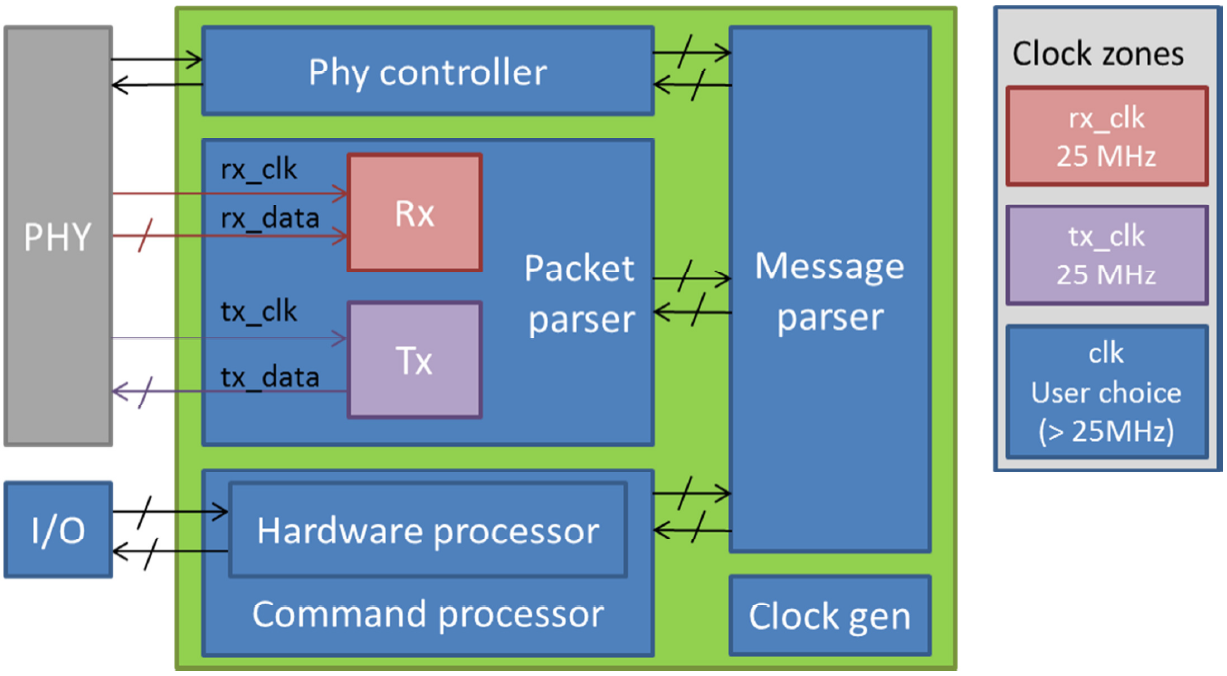
\includegraphics[width=0.6\linewidth]{IMG/ch4/PHY100}
		\caption{GbPhy firmware structure.}
		\label{fig:phy100}
	\end{figure}
	\noindent GbPhy provides a UDP-based Ethernet control link based on a fixed length 8 byte protocol (64 bit).
	For each 64~bit message the user can send 32~bit of data. The data are packed as follow:
	\begin{itemize}
		\item command\_contents(31 downto 28) => sub-system target:
		\newline
		for this application this can be \textit{0x1} for hardware commands, \textit{0x2} for LCD commands and \textit{0x4} for Tera10 commands.
		\item command\_contents(27 downto 20) => sub-system command identifier (ID):
		\newline
		each task (or command) is associated to a 8~bit number, an example of this is the list of commands in the \textit{Tera10 Controller} part in the next pages.
		\item command\_contents(19 downto 0) => sub-system command data:
		\newline
		these 20~bits are the data to be communicated or returned by the firmware; for example, this can be the value of a DAC that needs to be set, a list of channels that the user wants to enable or the value of a counter that the user want to read. 
	\end{itemize} 
	%%%%%%%%%%%%%%%%%%%%%%%%%%%%%%%%%%%%%%%%%%%%%%%%%%%%%%%%%%%%%%%%%%%%%%%%%% 
	\item \textbf{Command Processor}: this module is mainly a wrapper for every module that will be presented from now on. It also 
	redirects the commands according to the sub-system target.
	%%%%%%%%%%%%%%%%%%%%%%%%%%%%%%%%%%%%%%%%%%%%%%%%%%%%%%%%%%%%%%%%%%%%%%%%%%
	\item \textbf{LCD Controller}: it is the module that drives the 16x2 LCD display of the board.
	\begin{figure}[H]
		\centering
		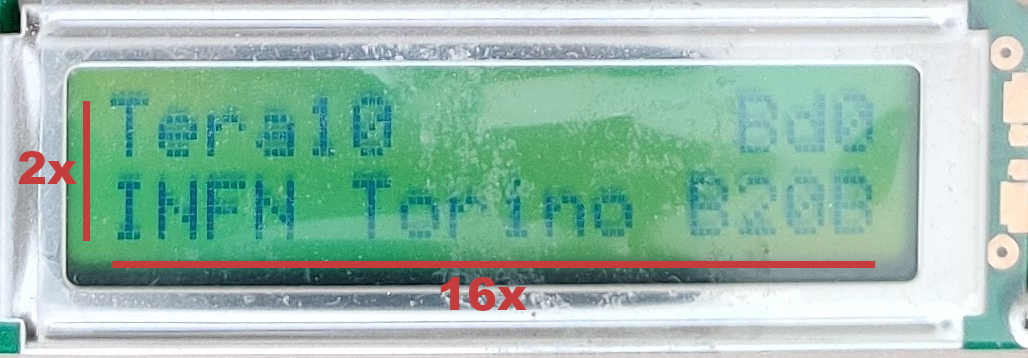
\includegraphics[width=0.5\linewidth]{IMG/ch4/LCD}
		\caption{KC705 tera10 LCD output.}
		\label{fig:lcd}
	\end{figure}
	\noindent This module contains multiple processes, FSMs (Finite State Machines) and a RAM module. The first FSM manages the start-up sequence for the LCD, the second does the conversion of the firmware version from hex to ASCII, a third one sends one by one the characters to the display while a fourth one manages the communications with the UDP module. In fact the firmware can not only display a fixed pre-selected banner, but also a user-sent 'message' from the pc.
	The LCD is extremely useful when working with multiples FPGAs to distinguish one board from the others or to keep track of the firmware version of each device.
	%%%%%%%%%%%%%%%%%%%%%%%%%%%%%%%%%%%%%%%%%%%%%%%%%%%%%%%%%%%%%%%%%%%%%%%%%%    
	\item \textbf{Tera10 I/O}: this module contains the declaration and port-map for 24 \textit{tera10 channel coincidence} modules~\cite{limardi}; each module receives as an input the data from two channels of the ABACUS2 chip, this signal is then de-serialized with a 1~GHz frequency clock (\textit{serdes\_clk}), ten times higher than the main clock (100~MHz). The output of the de-serializer is a 10~bit bus (one for each signal) to which it is added, using a shift register, the last bit from the previous bus. This is done in order to not lose any transition (high/low) from one packet and the next one when the number of pulses is counted from the number of the transitions.
	\newline
	The counting of the number of pulses is done with a LUT (Look Up Table) that from a 11~bit bus gives back a 3~bit logic vector corresponding to the number of transitions from 0 to 1. This result is used to update a 32~bit counter for each channel with the total number of pulses; in figure \ref{fig:coincidence} those are N1 for ch0 and N2 for ch1.
	\newline
	In order to count with efficiency even at high rates correction algorithms, based on the AND and OR combinations of the 10-bit words from to neighbouring channels, were implemented, and the corresponding number of transitions are counted using LUTs similar to the ones used to count the number of transitions in the two individual channels. The results are then added to four new 32~bit counters ($N_{AND}$, $T_{AND}$, $N_{OR}$ and $T_{OR}$). 
	\begin{figure}[H]
		\centering
		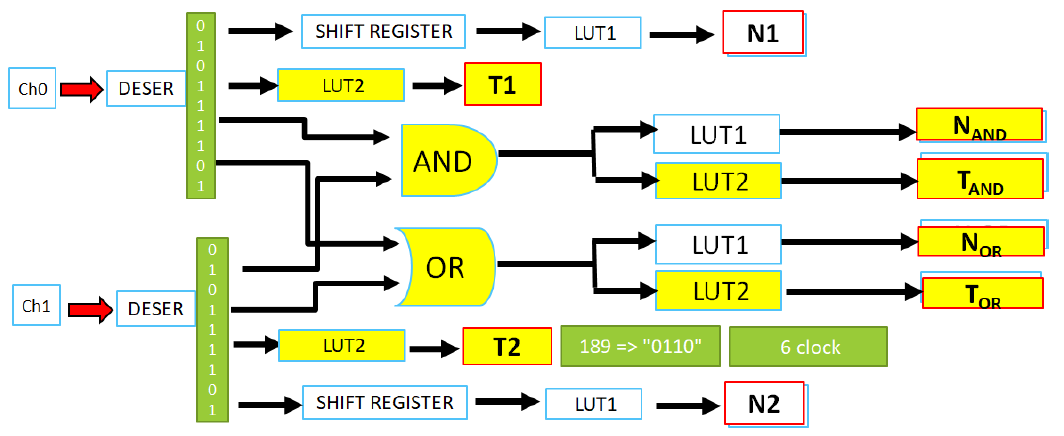
\includegraphics[width=0.7\linewidth]{IMG/ch4/COINCIDENCE}
		\caption{KC705\_tera10 channel coincidence architecture diagram.}
		\label{fig:coincidence}
	\end{figure}
	\noindent The counters $T_{1}$, $T_{2}$, $T_{AND}$ and $T_{OR}$ contain the number of clock strokes in which one of the two channel or a logic combination of both is \textit{high}.
	%%%%%%%%%%%%%%%%%%%%%%%%%%%%%%%%%%%%%%%%%%%%%%%%%%%%%%%%%%%%%%%%%%%%%%%%%% 
	\item \textbf{Tera10 Controller}: this module is strictly connected to the previous one (\textit{Tera10 I/O}). It receives the content of each counter from the previous block and manages the data according to the commands sent by the user. Some of the most used and important commands are:
	\begin{itemize}
		\item \textit{0x01} => \textit{reset serdes}: send reset signal for the de-serializers;
		\item \textit{0x02} => \textit{reset counters}: every counter for each \textit{tera10 channel coincidence} module is set to 0;
		\item \textit{0x10} => \textit{set counter enable}: to enable selected counters. This is done by dividing the channels in blocks of 16. When a 20~bit data command is sent, bits 18-17-16 are used to identify the block, and the next 16~bit are encoded one-hot for each channel; for example, to enable channel 2 the data to be sent is \textit{0-000-0000000000000010} and to enable channel 18 the data is \textit{0-001-0000000000000100};  
		\item \textit{0x11} => \textit{read counter}: read selected counter. the firmware response is a 16~bit bus, thus 2 commands are needed in order to read the entire counter; the LSB (Least Significant Bit) selects between the first and last 16~bit. For example:
		\newline
		fifo\_data(7 downto 0) = \textit{01110110} means read ch59\_counter(15 downto 0)
		\newline
		fifo\_data(7 downto 0) = \textit{01110111} means read ch59\_counter(31 downto 15)
		\item \textit{0x13} => \textit{read clocks}: read selected clock counter; the firmware response is a 16~bit bus, thus are valid the same considerations as before;
		\item \textit{0x14} => \textit{read coincidence counter}: read selected coincidence counter, the MSB (Most Significant Bit) selects between \textit{AND} and \textit{OR} counters; the firmware response is a 16~bit bus. For example:
		\newline
		fifo\_data(7 downto 0) = \textit{10000010} means read ch0203\_or\_counter(15 downto 0)
		\item \textit{0x15} => \textit{read coincidence clocks}: read selected clock coincidence counter, the MSB selects between \textit{AND} and \textit{OR} counters; the firmware response is a 16~bit bus as shown for command \textit{0x14};
		%\item x"18" \textit{set selected channel}:
		%\item x"20" \textit{do external trigger}:
		%\item x"12" \textit{read event buffer ram address}:
		%\item x"80" \textit{read event buffer ram}:
	\end{itemize}
	
	%%%%%%%%%%%%%%%%%%%%%%%%%%%%%%%%%%%%%%%%%%%%%%%%%%%%%%%%%%%%%%%%%%%%%%%%%% 
	\item \textbf{Hardware Controller}: this module manages hardware devices such as internal and external DACs, LEDs and GPIO (General Purpose Input Output) switches and buttons available on the FPGA board. The main commands are:
	\begin{itemize}
		\item \textit{0x01} => \textit{read GPIO switches}: this command returns the current state of the GPIO switches and buttons, thus:
		\newline
		reply(8 downto 4) = buttons state
		\newline
		reply(3 downto 0) = switches state
		\item \textit{0x02} => \textit{set hardware LED}: this command can turn on or off LEDs on the board;
		\item \textit{0x11} => \textit{set baseline DACs}: this command is used for both writing (setting) and reading the values of the ABACUS2 internal DACs, as explained in section \ref{InternalDac};
		%\item {\color{red} non so se ho detto cose sbagliate}
		\item \textit{0x20} => \textit{clear external DAC}: to clear the current settings of the eternal DAC;
		\item \textit{0x21} => \textit{set external DAC data register}: to set the external DAC with the values written in the RAM;
		\item \textit{0x22} => \textit{write external DAC register}: to write on memory the values to be written on the eternal DAC;
	\end{itemize}  
		
\end{itemize}
\noindent Each module contains at least two Finite State Machines (FSMs) in order to properly communicate with GbPhy and the logic needed to execute its purpose. The first FSM, in figure \ref{fig:fsmFIFO1}, reads a FIFO (First Input First Output) memory in which the commands received from GbPhy are stored. If the memory is empty the logic remains in the \textit{Idle} state until a new command is received. Once the command is selected the logic can execute it and generates a reply string.
\begin{figure}[H]
	\centering
	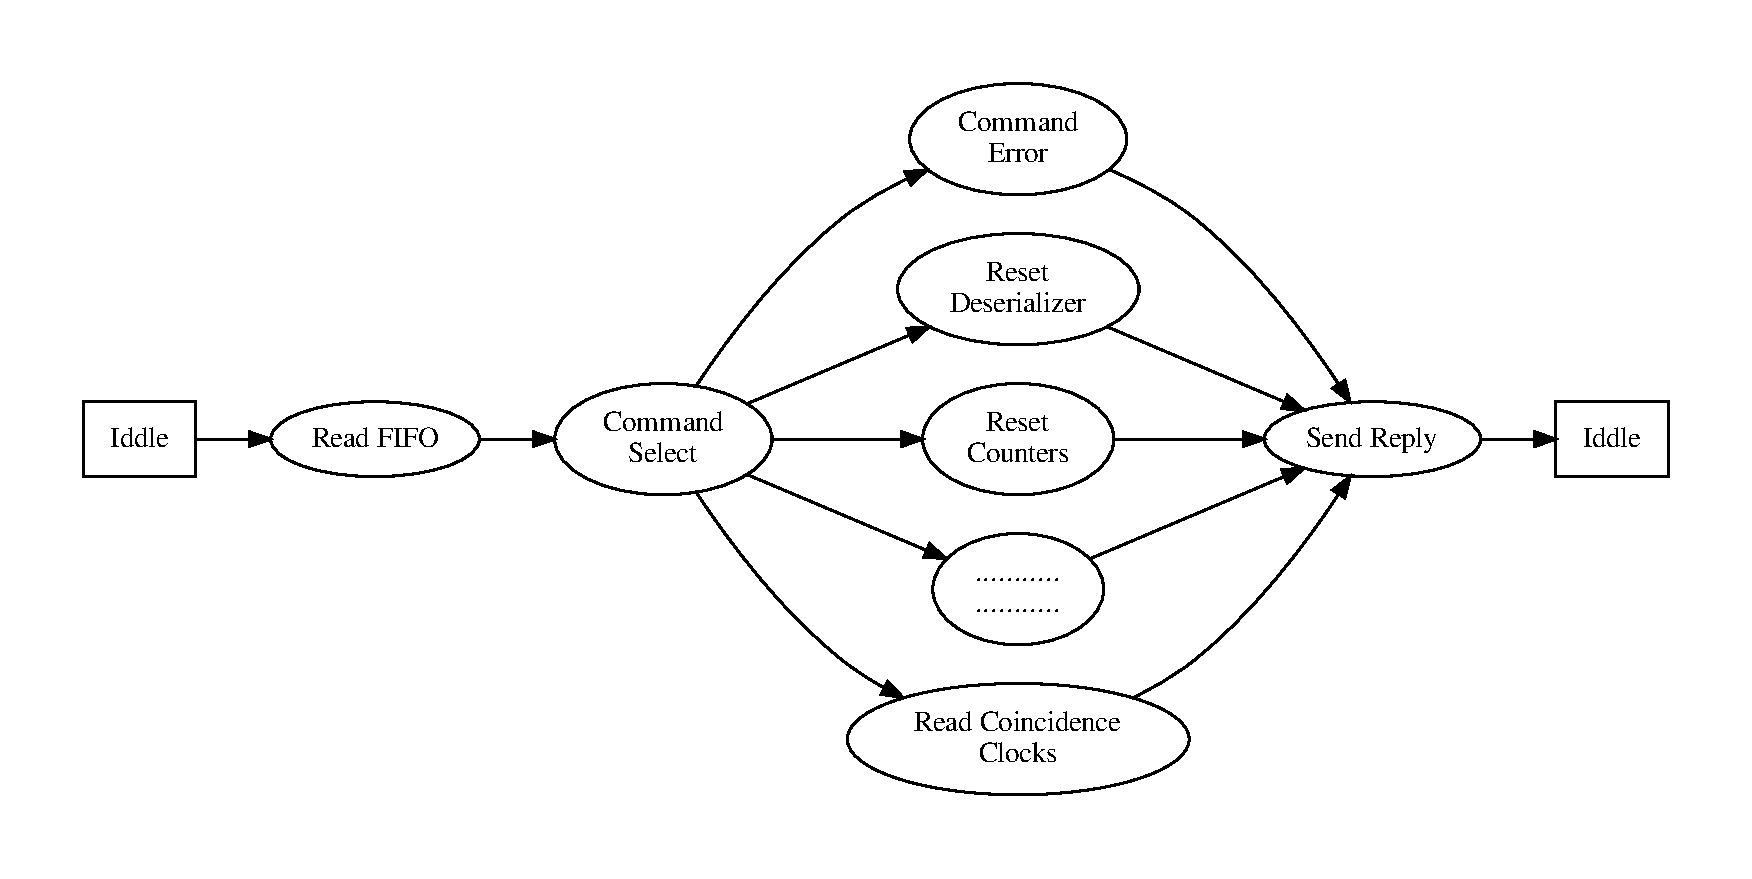
\includegraphics[width=1.0\linewidth]{FSMdiagrams/CMDtoTERA10.pdf}
	\caption{\textit{Command to TERA10} Finite State Machine diagram.}
	\label{fig:fsmFIFO1}
\end{figure}
\noindent In order to send the data to the computer in the correct order, another FIFO memory is implemented for storing all the replies strings.
The logic implemented to write the data into the memory is described in the FSM in figure \ref{fig:fsmFIFO2}.
%This is done in the \textit{Send Reply} state.
\begin{figure}[H]
	\centering
	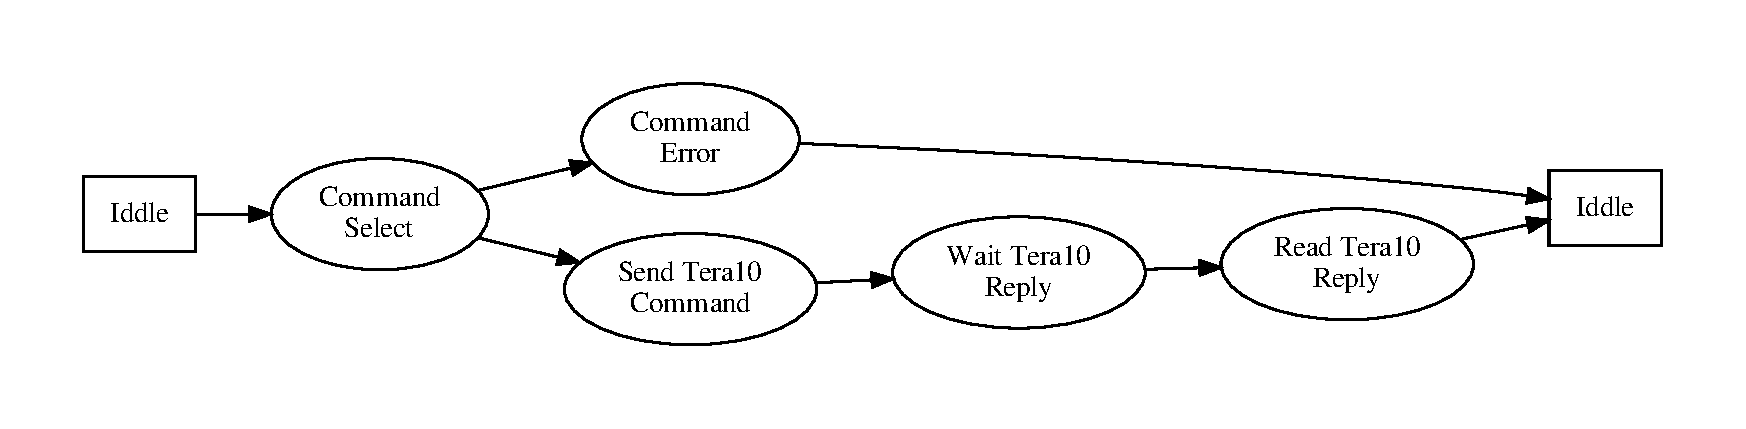
\includegraphics[width=1.0\linewidth]{FSMdiagrams/TERA10controll.pdf}
	\caption{\textit{TERA10 control} Finite State Machine.}
	\label{fig:fsmFIFO2}
\end{figure}  

\section{Firmware update}
My work on the KC705 firmware can be divided into three parts:
\begin{itemize}
	\item The implementation of the logic for the configuration of the ABACUS2 internal DACs, described in section \ref{InternalDac}. 
	\item The addition of a latch logic in order to save into a register the current value of every counter in the firmware, described in section \ref{Latch}.
	\item The addition of a timestamp generator to obtain a more precise calculation of the hit rate, described in section \ref{Timestamp}. 
\end{itemize}

\subsection{Hardware controller}\label{InternalDac}
\noindent The internal DACs of the ABACUS2 chip are configured using an on-chip I2C controller (figure \ref{fig:internaldac}), a module with 3 inputs (Serial Clock, Serial INput and Reset) and an output (Serial OUTput)~\cite{dac}.
The controller behaviour is simulated using a Verilog module.
%The tests therefore simulate not only the firmware operation, but also the response of the chip itself.
\begin{figure}[H]
	\centering
	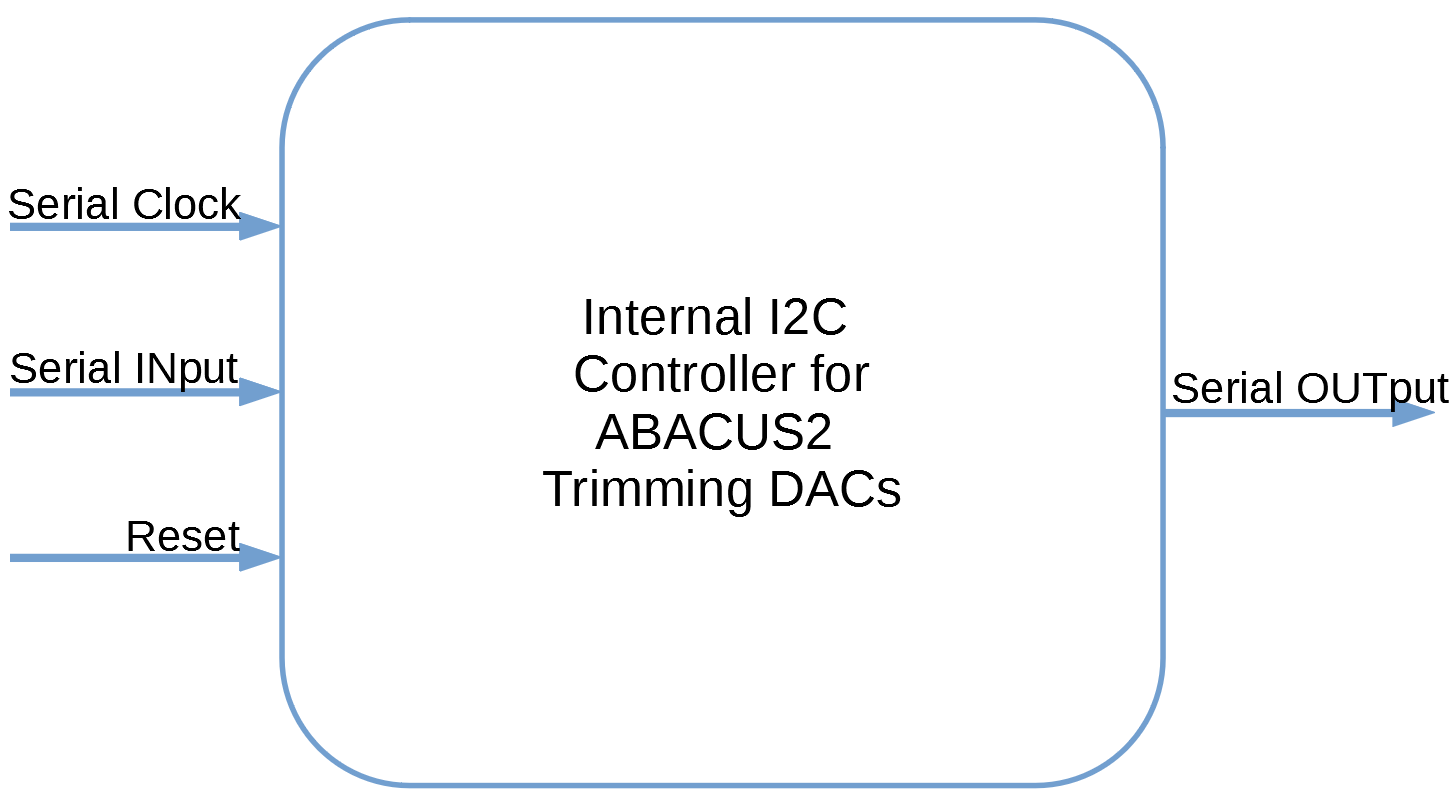
\includegraphics[width=0.34\linewidth]{IMG/ch4/INTERNALDAC.PNG}
	\caption{Diagram of internal I2C controller for trimming DACs configuration.}
	\label{fig:internaldac}
\end{figure}
\noindent The 24 threshold fine tuning DACs are controlled by 24 5-bits registers. These registers can be independently
loaded and read-out via a serial interface protocol based on 16-bits words. The commands are send via a Serial
INput pin (SIN) and the data are read-out on a Serial OUTput pin (SOUT). The two serial streams are
synchronous to the clock input (CLK) and are sampled on the clock rising edge.
The write operations are performed according to the following sequence:
\begin{itemize}
	\item Send start sequence : 0xA5A5 = 0b\textit{1010010110100101}
	\item Send write command : \textit{11}a$_{13}$a$_{12}$a$_{11}$a$_{10}$a$_{9}$a$_{8}$d$_{7}$d$_{6}$d$_{5}$d$_{4}$d$_{3}$d$_{2}$d$_{1}$d$_{0}$ with:
	\begin{itemize}
		\item \textit{11} = write command
		\item a$_{13}$ $\rightarrow$ a$_{8}$ = 6~bit address. a$_{13}$ $\rightarrow$ a$_{9}$ is the channel address (with reference to the physical layout (figure \ref{fig:abacus2}), address 0 is the leftmost channel and 23 is the rightmost one), while a$_{8}$ selects the VTH+ (when 1) or the VTH- DAC (when 0); this function is not used for this version of the ABACUS chip. Addresses from 24 to 31 are not used.
		\item d$_{7}$ $\rightarrow$ d$_{0}$ = 8~bit data. The bits d$_{5}$ $\rightarrow$ d$_{0}$ are the data to be written in the DAC registers (from 0 to 63)to set the threshold voltage; the remaining two MSBs (d$_{7}$d$_{6}$) are not used.
	\end{itemize}
\end{itemize}
\noindent The read operations are performed as follows :
\begin{itemize}
	\item Send start sequence : 0xA5A5 = 0b\textit{1010010110100101}
	\item Send read command : \textit{10}a$_{13}$a$_{12}$a$_{11}$a$_{10}$a$_{9}$a$_{8}$00x$_{5}$x$_{4}$x$_{3}$x$_{2}$x$_{1}$x$_{0}$ with:
	\begin{itemize}
		\item \textit{10} = read command
		\item a$_{13}$ $\rightarrow$ a$_{8}$ = 6~bit address.
		\item 00x$_{5}$ $\rightarrow$ x$_{0}$. With x = DON'T CARE 
	\end{itemize}
	\item The serial output is a 16 bits word with format \textit{11}a$_{13}$a$_{12}$a$_{11}$a$_{10}$a$_{9}$a$_{8}$00d$_{5}$d$_{4}$d$_{3}$d$_{2}$d$_{1}$d$_{0}$ with:
	\begin{itemize}
		\item \textit{11} = response of successful reading.
		\item a$_{13}$ $\rightarrow$ a$_{8}$ = confirmation of the reading address.
		\item d$_{5}$d$_{4}$d$_{3}$d$_{2}$d$_{1}$d$_{0}$ = 6~bit word of data.
	\end{itemize}
\end{itemize}
\noindent After any operation (write or read) send a \textit{00}x$_{13}$x$_{12}$x$_{11}$x$_{10}$x$_{9}$x$_{8}$x$_{7}$x$_{6}$x$_{5}$x$_{4}$x$_{3}$x$_{2}$x$_{1}$x$_{0}$. With x = DON'T CARE
\subsubsection{Configuration logic}\label{confing}
In order to configure the internal DACs of the ABACUS2 chip 16~bits words are needed. The UDP protocol implemented with the GbPhy project gives the user the possibility to send 20~bits of data.
Therefore the data bits were divided as follows:
\begin{itemize}
	\item 3 bits ( data19 $\rightarrow$ data17 ) not used
	\item 2 bits ( data16 $\rightarrow$ data15 ) command
	\item 6 bits ( data14 $\rightarrow$ data9 ) address
	\item 8 bits ( data8 $\rightarrow$ data1 ) DAC data
	\item 1 bit ( data0 ) DAC select
\end{itemize}
\noindent The pre-existing hardware controller module had a command and a logic for the configuration of the internal DACs of the first version of the ABACUS chip.
In this version of the chip the DAC configuration was based on a long shift-register that did not worked properly due to timing issues.
I decided to maintain the same sub-system command ID of the previous version and completely rewrite the FSM that sends the data. 
In figure \ref{fig:fsmDACs} the new logic diagram of the implemented FSM is shown.
\begin{figure}[H]
	\centering
	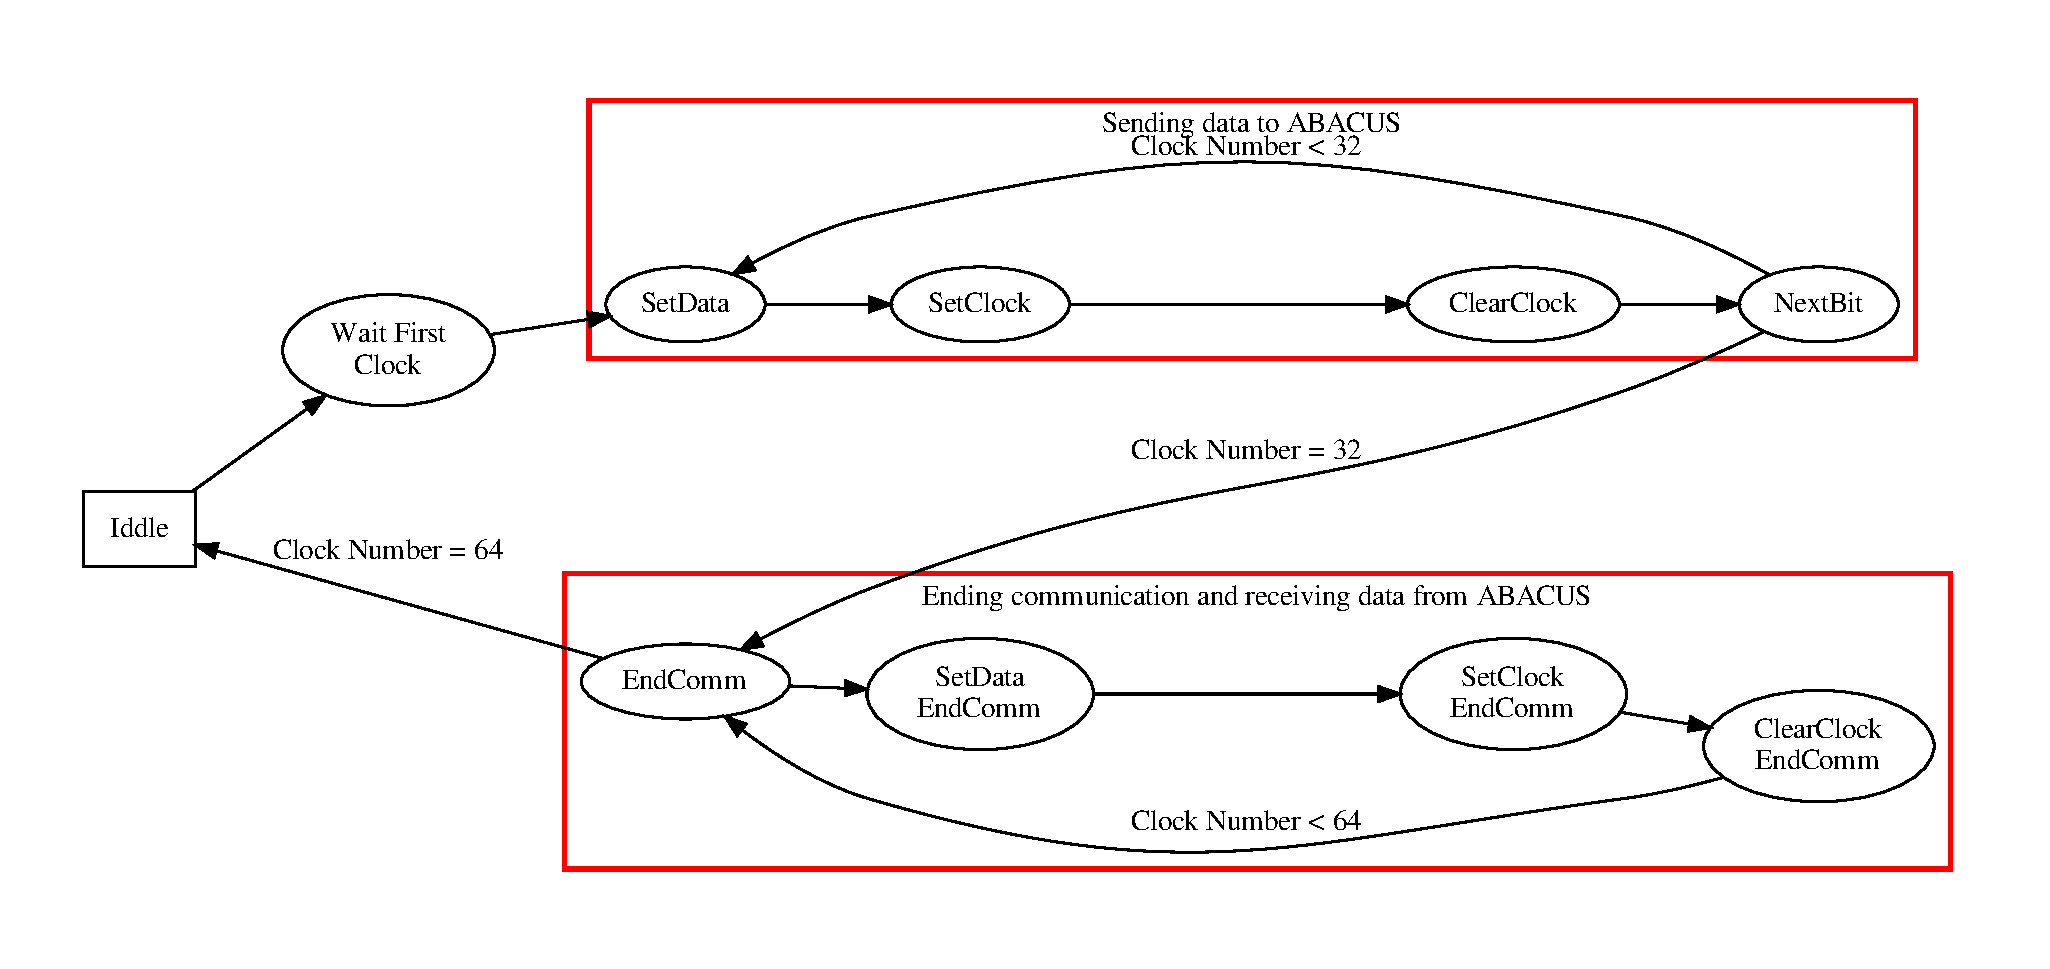
\includegraphics[width=1.0\linewidth]{FSMdiagrams/InternalDACsFSM.pdf}
	\caption{FSM for the configuration of the internal fine tuning DACs of the ABACUS2 chip.}
	\label{fig:fsmDACs}
\end{figure}
\noindent The FSM runs into an independent process that sends to the chip 64 clock strokes; in the first 32 the data are sent, while in the remaining 32 the firmware is waiting for a response from the the ASIC.
In figure \ref{fig:fsmDACs} the two operations are divided into two red clusters.
By examining the finite state machine the following states are observed:
\begin{itemize}
	\item \textbf{Idle}: when an internal DAC configuration command is received the logic of the FSM in figure \ref{fig:fsmFIFO1} will turn \textit{high} a signal in order to trigger this process (\textit{set\_baseline\_dacs}), thus the state of this machine will go from \textit{Idle} to \textit{WaitFirstClock} on the first rising edge of the 125~MHz clock.
	\begin{figure}[H]
		\centering
		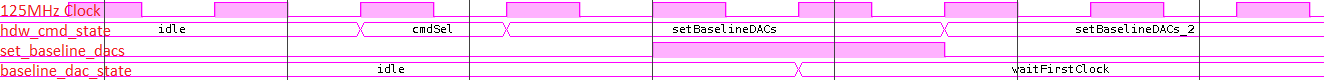
\includegraphics[width=1.0\linewidth]{IMG/ch4/DACsimulations/FSMiddle}
		\caption{}
		\label{fig:fsmiddle}
	\end{figure} 
	\item \textbf{Wait first clock}: in order to generate the \textit{sck} (serial clock for the internal DACs) the logic uses a 12~bit (\textit{baseline\_clk\_div\_ctrl}) counter that generates a signal (\textit{baseline\_clk\_div}) each time it is full, thus it counts \textit{FFF}.
	\newline It can be noted that the state of the \textit{baseline\_dac\_state} does not change immediately after the counter reaches \textit{0xFFF}, but this is not a problem since this delay is always the same and it does not affect the logic.
	\newline The process that runs the counter is independent from the FSM, it runs always. In order to synchronize the counter and the logic an additional state that waits until the counter resets to 0 was implemented, as shown in figure \ref{fig:fsmwaitfirstclock}. 
	\begin{figure}[H]
		\centering
		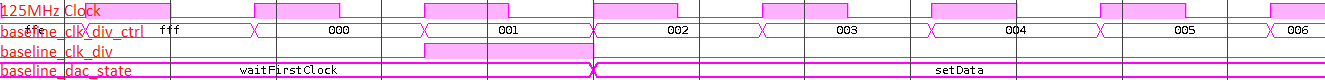
\includegraphics[width=1.0\linewidth]{IMG/ch4/DACsimulations/FSMwaitfirstclock}
		\caption{}
		\label{fig:fsmwaitfirstclock}
	\end{figure}
	\item \textbf{Set Data}: with the first \textit{setData} state it starts the first cluster (sending data to the chip).
	The initial 16~bits are coded into the firmware and are always the same \textit{0xA5A5}.
	The \textit{setData} state waits until a \textit{baseline\_clk\_div} signal (when the counter resets) is \textit{high} and then drives the \textit{baseline\_dac\_mosi} (Master Output Slave Input) signal that sends data from the FPGA to the chip accordingly to the received command.
	When the signal is sent the FSM also change state to \textit{setClock}.
	This can be seen in figure \ref{fig:fsmsetdata}. 
	\begin{figure}[H]
		\centering
		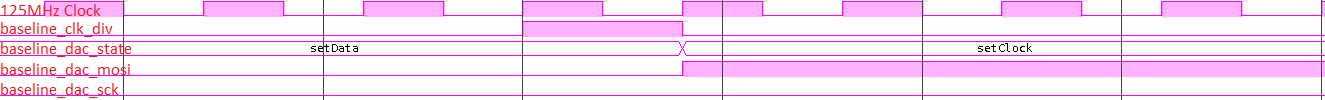
\includegraphics[width=1.0\linewidth]{IMG/ch4/DACsimulations/FSMsetdata}
		\caption{}
		\label{fig:fsmsetdata}
	\end{figure}
	\item \textbf{Set Clock}: the generation of the \textit{baseline\_dac\_sck} works on the same principle. When the counter resets the FSM changes state and the clock output is driven \textit{high}.
	\begin{figure}[H]
		\centering
		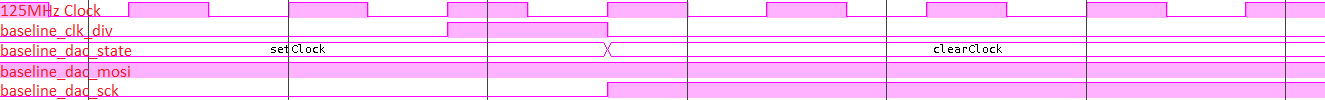
\includegraphics[width=1.0\linewidth]{IMG/ch4/DACsimulations/FSMsetclock}
		\caption{}
		\label{fig:fsmsetclock}
	\end{figure}
	\item \textbf{Clear Clock}: The clock signal is now \textit{high} and the data was previously setted, thus it can be assumed that the chip sampled correctly the information. At this point, again, when the counter resets itself, the FSM changes state and the clock signal goes \textit{low}.
	\newline It is important to observe that from the end of \textit{setClock} to the end of \textit{clearClock} 1 counter cycle is required, however from the end of \textit{clearClock} to the end of \textit{setClock} 2 counter cycles are needed. This leads to a clock signal with 33\% duty cycle that is perfectly fine for the ABACUS2 chip.
	The FSM clock has a 8~ns period, the counter has 12~bits and resets itself when it is full. Thus, since 0xFFF~=~4095, it can be calculated that a counter cycles lasts 32.76~$\mu$s~=~8~ns$\cdot$4095. The theoretic clock period of the internal DACs should be three times this value, therefore 98.28~$\mu$s. It will be shown if section \ref{dactests} that this is perfectly correct.     
	\begin{figure}[H]
		\centering
		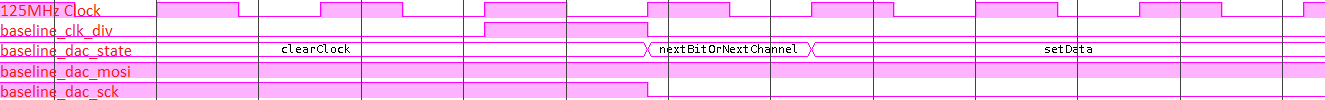
\includegraphics[width=1.0\linewidth]{IMG/ch4/DACsimulations/FSMnextbit}
		\caption{}
		\label{fig:fsmnextbit}
	\end{figure}
	\item \textbf{Next Bit}: inside the FSM there is a 5~bit counter (\textit{baseline\_dac\_bit\_ctrl}) that keeps trace of the number of bits sent to the chip. The \textit{nextBit} state checks this value; if the number of clocks (data in) is less than 32 the logic keeps sending data, as shown in figure \ref{fig:fsmcluster1}, while if the number of clocks is 32 the logic start the \textit{ending communication} sequence, as in figure \ref{fig:fsmendcommunication}.
	\begin{figure}[H]
		\centering
		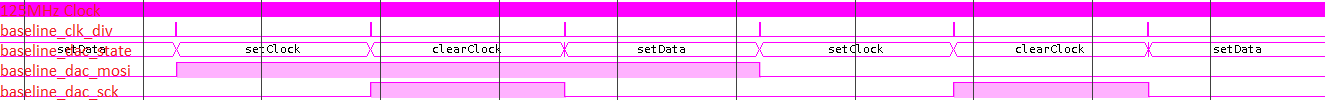
\includegraphics[width=1.0\linewidth]{IMG/ch4/DACsimulations/FSMcluster1}
		\caption{}
		\label{fig:fsmcluster1}
	\end{figure}
	\item \textbf{End Communication}: the \textit{EndCommunication} state starts the second cluster of the FSM in figure \ref{fig:fsmDACs} (ending communication and receiving data from ABACUS2). This state performs the same tasks as \textit{nextBit}; it checks if \textit{baseline\_dac\_bit\_ctrl}<32.
	If the condition is true the logic switches to \textit{SetDataEndCommunication}, if the condition is false the logic returns to idle. 
	\begin{figure}[H]
		\centering
		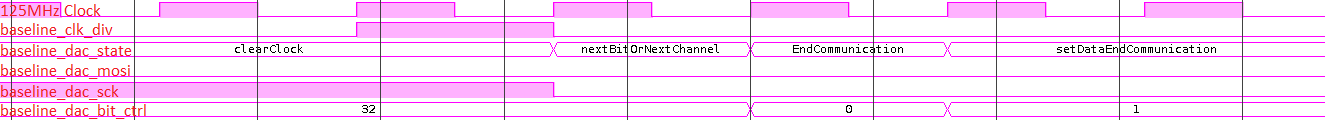
\includegraphics[width=1.0\linewidth]{IMG/ch4/DACsimulations/FSMendcommunication}
		\caption{}
		\label{fig:fsmendcommunication}
	\end{figure}
	\item \textbf{Set Data End Communication}: this state keeps the output (\textit{baseline\_dac\_mosi} = Data INput) always \textit{low}.
	\begin{figure}[H]
		\centering
		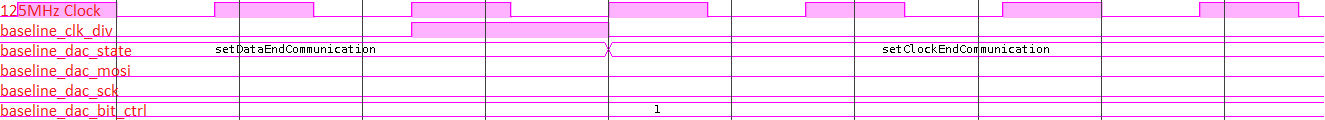
\includegraphics[width=1.0\linewidth]{IMG/ch4/DACsimulations/FSMsetdataendcommunication}
		\caption{}
		\label{fig:fsmsetdataendcommunication}
	\end{figure}
	\item \textbf{Set Clock End Communication}: as for the \textit{setClock} state, when the 12~bit counter resets it drives \textit{high} the ABACUS2 clock signal.
	\begin{figure}[H]
		\centering
		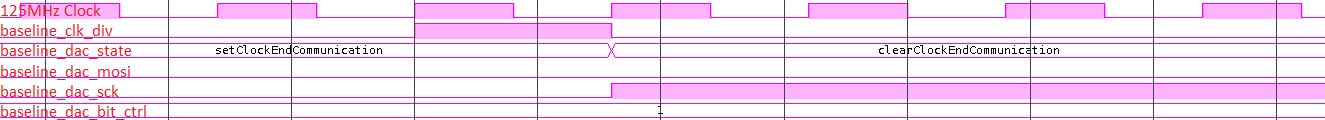
\includegraphics[width=1.0\linewidth]{IMG/ch4/DACsimulations/FSMsetclockendcommunication}
		\caption{}
		\label{fig:fsmsetclockendcommunication}
	\end{figure}
	\item \textbf{Clear Clock End Communication}: as for the \textit{clearClock} state, when the 12~bit counter resets it drives \textit{low} the ABACUS2 clock signal.
	\begin{figure}[H]
		\centering
		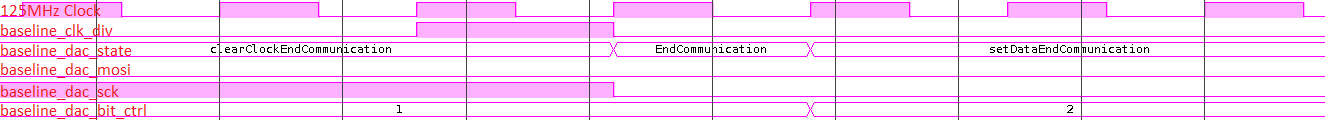
\includegraphics[width=1.0\linewidth]{IMG/ch4/DACsimulations/FSMclearclockendcommunication}
		\caption{}
		\label{fig:fsmclearclockendcommunication}
	\end{figure}	
\end{itemize}

\noindent Figure \ref{fig:fsmalmostall} shows an overview of the data sent to the chip. On the second row there is the \textit{baseline\_clk\_div} signal that goes \textit{high} when the 12~bit counter resets. On row number three it can bee seen the \textit{baseline\_dac\_mosi} signal; these are the configuration bits sent to the chip. It should be noted that the first 16~bits are the start sequence \textit{1010-0101-1010-0101}.
Row number four shows the \textit{baseline\_dac\_sck} signal; it has to be noted that the duty cycle is 33\% and that the transitions of the \textit{baseline\_dac\_mosi} signal are always shifted by $\approx$33~$\mu$s compared to those of the clock.
This ensures that the signal is stable before sampling.
The fifth row contains the value of the \textit{baseline\_dac\_bit\_ctrl} counter; it has to be noted that it resets after the value of 32 and after that the MOSI signal is always \textit{low}.   
\begin{figure}[H]
	\centering
	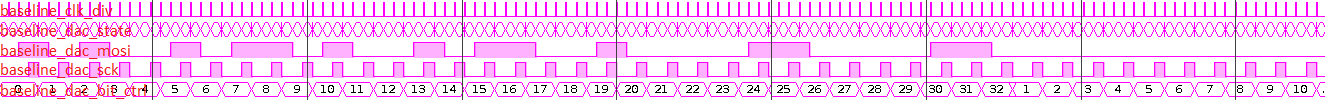
\includegraphics[width=1.0\linewidth]{IMG/ch4/DACsimulations/FSMalmostall}
	\caption{}
	\label{fig:fsmalmostall}
\end{figure}
\subsubsection{Reading logic}
In order to read the data from the chip I implemented two new processes: a 16~bit shift register (\textit{shift\_register\_baseline\_dac(15 downto 0)}) and a comparator.
The shift register receives the MISO (Master Input Slave Output) signal and samples it at the falling edge of the \textit{baseline\_dac\_sck} signal. Then it stores the data into a bus that is updated at each clock stroke.
The comparator searches for the first 8~bits (the MSBs) of the shift register and compares them with the address of the received read command.
If \textit{shift\_register\_baseline\_dac(15 downto 8) = 11 + fifo\_data(14 downto 9)}, thus if the first 8 bits of the shift register are equal to 11+address as seen in section \ref{InternalDac}, then the remaining 8 bit of the shift register are the data of the internal DAC.
\begin{figure}[H]
	\centering
	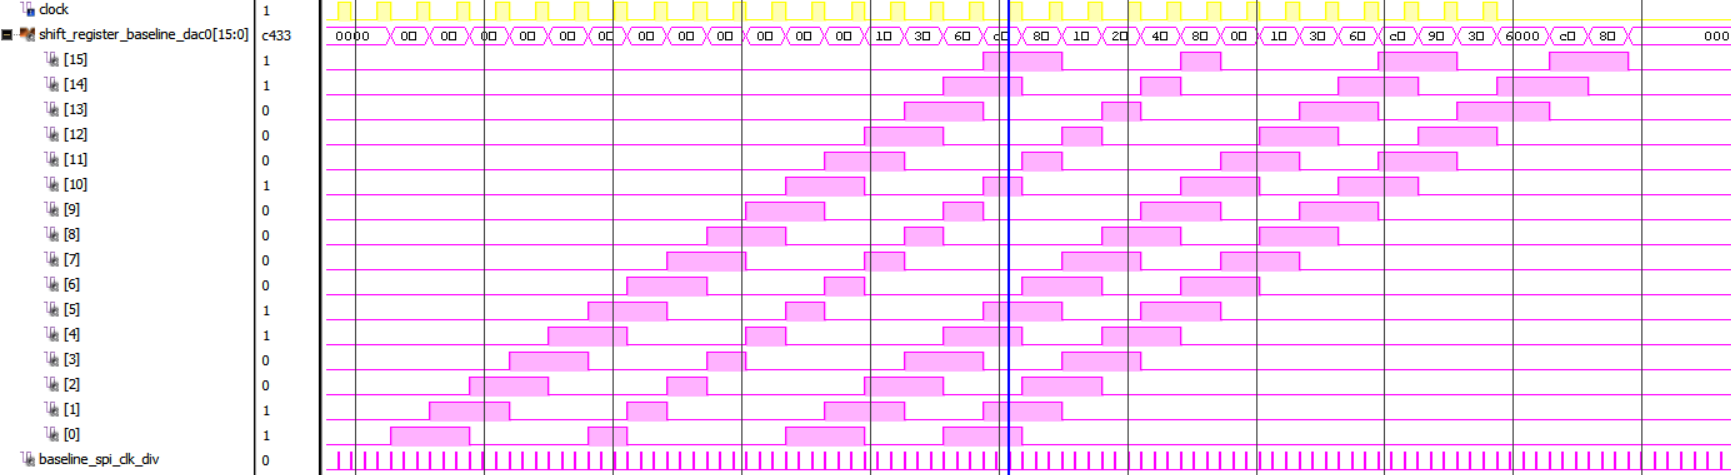
\includegraphics[width=1.0\linewidth]{IMG/ch4/DACsimulations/FSMshiftregister}
	\caption{}
	\label{fig:fsmshiftregister}
\end{figure}
\noindent In figure \ref{fig:fsmshiftregister} the read command was \textit{"000 "10" "000100" "00000000" "0"} (read command on channel 4 ) and it can be seen that when the first 8~bits of the shift register are \textit{"11000100"} the last 8 bits are the data, in this case \textit{"00110011"}~=~\textit{0x33}.
On board tests will be analysed  in section \ref{dactests}.

%%%%%%%%%%%%%%%%%%%%%%%%%%%%%%%%%%%%%%%%%%%%%%%%%%%%%%%%%%%%%%%%%%%%%%%%%%%%%%%%%%%%%%
\subsection{Latching counters}\label{Latch}
\noindent In the original FPGA firmware any counter could be read in any moment, even while counting, but only one at the time.
This setup has some limitations, the main one being that the firmware could not read the value of two or more counters simultaneously.
In addition the clock of the PC used to collect the data was used to determine the count rate from two subsequent readings of the counters; this PC clock is not synchronous with the data collection time, giving rise to errors in the count rate measurement.
In order to solve the problem I implemented a latch system that saves into a memory the current state of every counter and generates a timestamp.
I thus created a new module, called \textit{tera10\_latch\_counter} that contains all the memory and the logic needed for the latch system and for the timestamp generation.
This part will be explained in section \ref{Timestamp}.
The firmware has a total of 192 counters that needs to be latched, which are divided as follows:
\begin{itemize}
	\item 48 hit counters
	\item 48 clock counters
	\item 48 AND/OR coincidence hit counters
	\item 48 AND/OR coincidence clock counters
\end{itemize}
\noindent Each channel needs to be saved at the same time (same clock stroke), thus a deep RAM block that contains every counter in a different address can not be taken into consideration.
I decided to compile a new Block RAM IP, as in figure \ref{fig:ramip}. This new pre-configured module implements an easy to use (32x2) RAM component, thus 32~bits of data and two possible states (1~bit address). The final version of the firmware will use 192 of this components.
This means that for each state a total of 6.144~kb of memory needs to be allocated, thus in total 12.288~kb; this is feasible and perfectly manageable by the KC705 board. 
\begin{figure}[H]
	\centering
	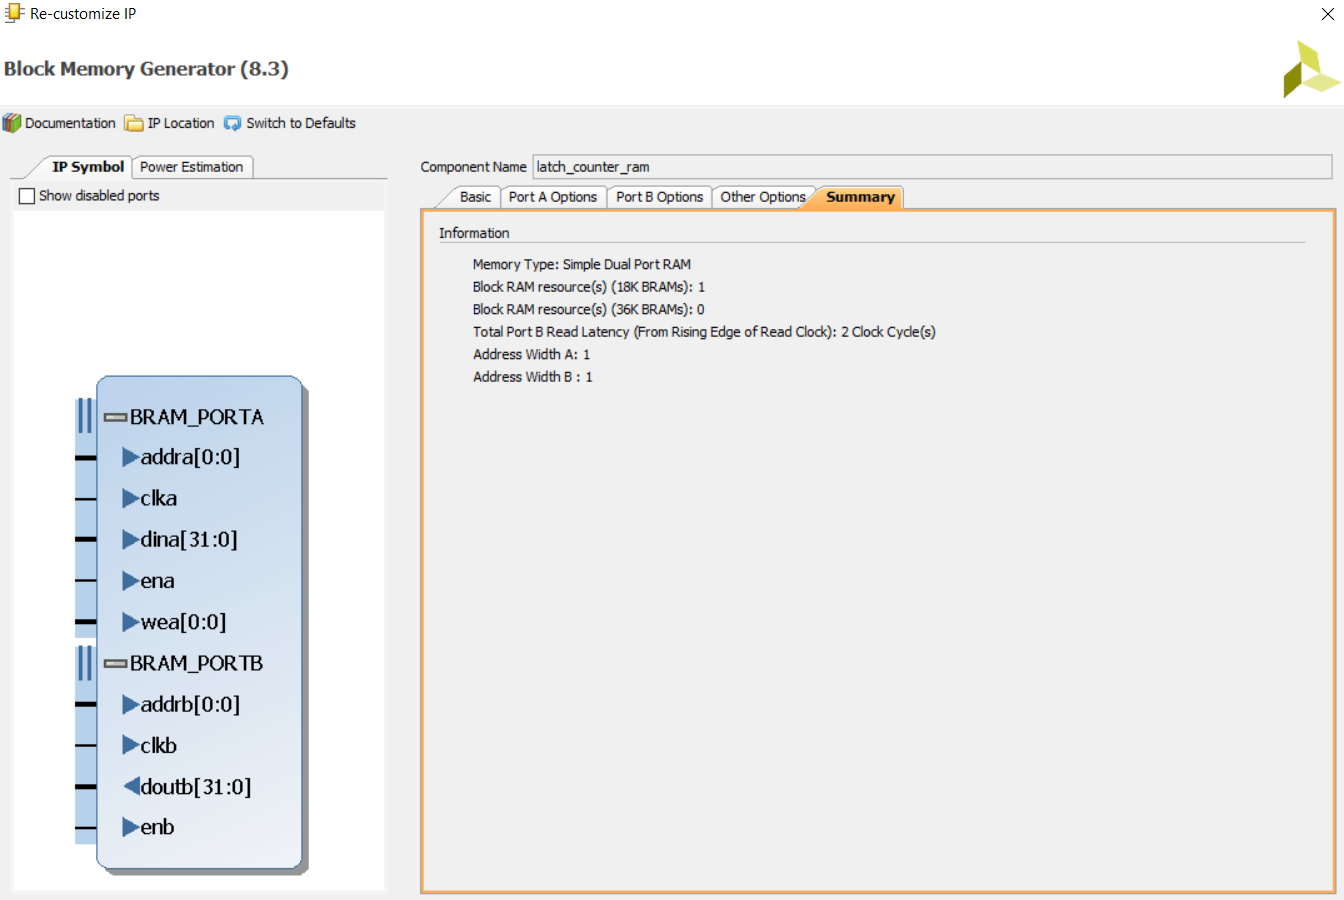
\includegraphics[width=0.5\linewidth]{IMG/ch4/LATCH_RAM_IP}
	\caption{Vivado IP manager summary for Latch Counters Block Memory IP.}
	\label{fig:ramip}
\end{figure}
\noindent Before talking about the latch logic it is important to understand how the RAM needs to be controlled. There are a total of 8 input signals and one output:
\begin{itemize}
	\item \textit{clka} and \textit{clkb}: clock signal for writing and reading logic. Considering that all the logic runs with the 125~MHz \textit{tera10\_clk}, in order to avoid timing errors \textit{clka} and \textit{clkb} will also have a frequency of 125~MHz
	\item \textit{ena} and \textit{enb}: enable signal for ram ports \textit{A} and \textit{B}, this signals are always \textit{high}
	\item \textit{dina}: 32~bit input signal
	\item \textit{doutb}: 32~bit output signal
	\item \textit{addra}: 1~bit write address, this means that the RAM has depth~=~2, thus two states can be latched
	\item \textit{addrb}: 1~bit read address
	\item \textit{wea}: \textit{write enable a}, when this signal is \textit{high} the input from dina is saved into memory at the address \textit{addra}
\end{itemize} 
\noindent The \textit{tera10\_latch\_counter} receives as inputs every counter from \textit{tera10\_I/O}; each counter is then routed to the input (\textit{dina}) of one RAM component. When the user sends a \textit{do\_latch} command with the desired address ('\textit{0}' or '\textit{1}') the \textit{wea} signal will turn \textit{high} for each RAM and thus the state of every counter will be saved.
\begin{figure}[H]
	\centering
	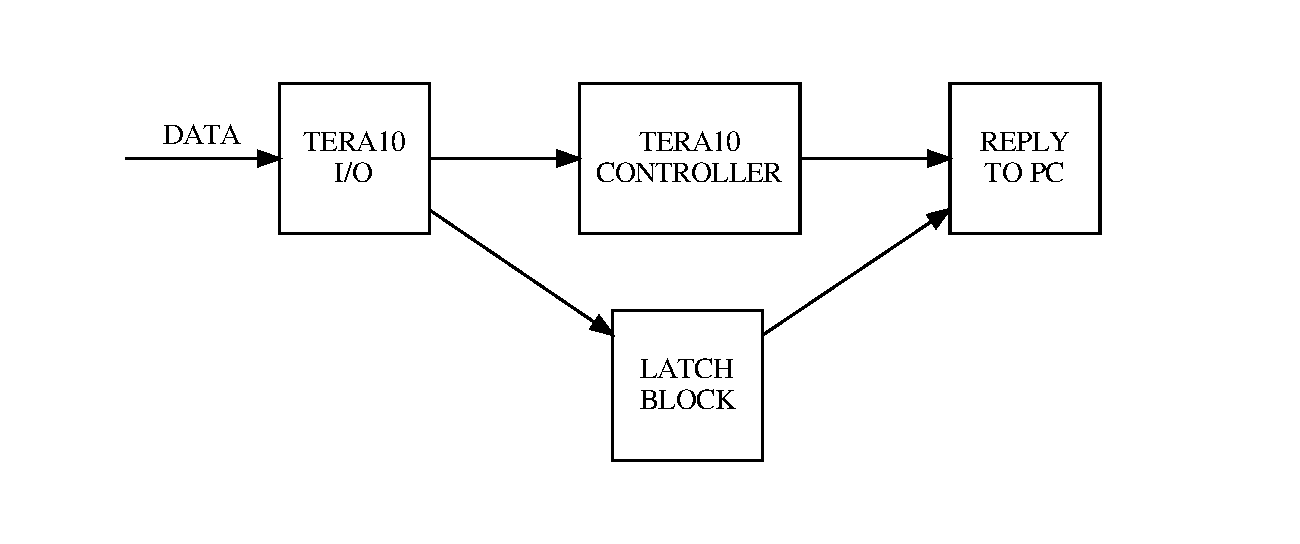
\includegraphics[width=0.7\linewidth]{FSMdiagrams/latch_counter.pdf}
	\caption{Counters data flow from \textit{tera10\_I/O} to the PC.}
	\label{fig:latch_counter}
\end{figure}
\noindent In order to control the block, I created a new sub-system target (\textit{0x8}) dedicated to the latch and timestamp and two new FSMs with the same style as the ones in figure \ref{fig:fsmFIFO1} and \ref{fig:fsmFIFO2}. The new sub-system commands ids are:
\begin{itemize}
	\item \textit{0x0F} => \textit{do latch}: 
	\begin{itemize}
		\item fifo\_data(8) = write address ('\textit{0}' or '\textit{1}')
	\end{itemize}
	\item \textit{0x1F} => \textit{read latch counters}:
	\begin{itemize}
		\item fifo\_data(8) = read address ('\textit{0}' or '\textit{1}')
		\item fifo\_data(7 downto 1) = counter select (from 0$\rightarrow$"\textit{0000000}" to 48$\rightarrow$"\textit{0110000}")
		\item fifo\_data(0) = bit select $\rightarrow$ read first or last 16 bits of the counters \\('0'$\rightarrow$read~15~downto~0; '1'$\rightarrow$read~31~downto~15)
	\end{itemize}
	\item \textit{0x2F} => \textit{read latch clocks}:
	\begin{itemize}
		\item fifo\_data(8) = read address ('\textit{0}' or '\textit{1}')
		\item fifo\_data(7 downto 1) = counter select (from 0$\rightarrow$"\textit{0000000}" to 48$\rightarrow$"\textit{0110000}")
		\item fifo\_data(0) = bit select $\rightarrow$ read first or last 16 bits of the counters \\('0'$\rightarrow$read~15~downto~0; '1'$\rightarrow$read~31~downto~15)
	\end{itemize}
	\item \textit{0x3F} => \textit{read latch coincidence counters}:
	\begin{itemize}
		\item fifo\_data(8) = read address ('\textit{0}' or '\textit{1}')
		\item fifo\_data(7) = coincidence select ('0'$\rightarrow$read AND coincidence; '1'$\rightarrow$read OR coincidence)
		\item fifo\_data(6 downto 1) = counter select (from 0$\rightarrow$"\textit{0000000}" to 24$\rightarrow$"\textit{0011000}")
		\item fifo\_data(0) = bit select $\rightarrow$ read first or last 16 bits of the counters \\('0'$\rightarrow$read~15~downto~0; '1'$\rightarrow$read~31~downto~15)
	\end{itemize}
	\item \textit{0x4F} => \textit{read latch coincidence clocks}:
	\begin{itemize}
		\item fifo\_data(8) = read address ('\textit{0}' or '\textit{1}')
		\item fifo\_data(7) = coincidence select ('0'$\rightarrow$read AND coincidence; '1'$\rightarrow$read OR coincidence)
		\item fifo\_data(6 downto 1) = counter select (from 0$\rightarrow$"\textit{0000000}" to 24$\rightarrow$"\textit{0011000}")
		\item fifo\_data(0) = bit select $\rightarrow$ read first or last 16 bits of the counters \\('0'$\rightarrow$read~15~downto~0; '1'$\rightarrow$read~31~downto~15)
	\end{itemize}
	\item \textit{0x5F} => \textit{do timestamp}: see section \ref{Timestamp}
	\item \textit{0x6F} => \textit{read timestamp}: see section \ref{Timestamp}
\end{itemize}

\subsubsection{Vivado simulations}
\noindent In order to test the correct functioning of the latch logic I performed extensive software simulations. In figure \ref{fig:dolatch} it can be seen how the latching system works for one channel, in this case \textit{ch00}. The first signal is the 125~MHz clock; the following 3 lines show the received packet divided in three buses:
\begin{itemize}
	\item fifo\_target = sub-system target, in this case \textit{0x8}
	\item fifo\_command = sub-system commands id, in this case \textit{0x0F}, corresponding to a \textit{do\_latch} command
	\item fifo\_data = command data, in this case \textit{0x00100}, only fifo\_data(8)=~'1'. This means that the data will be saved on address 1.
\end{itemize} 
The next signal is \textit{ch00\_data}, this is a 32~bit counter that contains the number of pulses that have been detected by the sensor (in this case 7).
The following row shows the state of the FSM that controls the latch module. It is interesting to observe how it works:
from the idle state the logic reads the FIFO memory that contains the command and stores it into a register, then the \textit{cmdSel} state drives the FSM to the appropriate next state using the command ID.
Once the FSM is in the \textit{DOlatch} state, the write enable signal (\textit{wea}) turns \textit{high} for one clock stroke and the address updates following the command data, in this case '\textit{1}'.  
\begin{figure}[H]
	\centering
	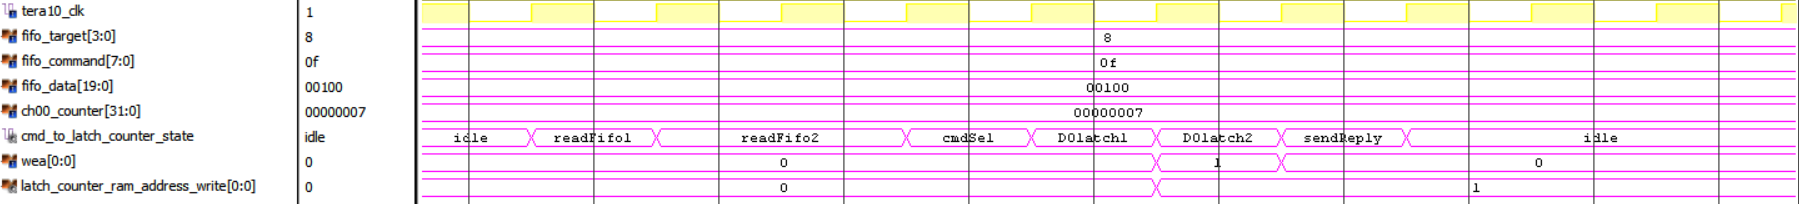
\includegraphics[width=1.0\linewidth]{IMG/ch4/LATCHsimulations/DOLATCH}
	\caption{}
	\label{fig:dolatch}
\end{figure}
\noindent Figure \ref{fig:readlatch} shows an example of the reading process from a RAM module. The first signal is the 125~MHz clock followed in the next row by the value of the received packet:
\begin{itemize}
	\item fifo\_target = sub-system target, in this case \textit{0x8}
	\item fifo\_command = sub-system commands id, in this case \textit{0x1F}, thus a \textit{read\_latch\_counter} command
	\item fifo\_data = command data, in this case \textit{0x00100}, only fifo\_data(8)=~'\textit{1}'. This means that the data will be read from address \textit{1}, from the channel \textit{0}, since fifo\_data(7 downto 1) = "\textit{0000000}" and from the first 16~bits since the least significant bit is \textit{0}.
\end{itemize}
\noindent When the FSM state is \textit{ReadLatchCounter}, the \textit{latch\_counter\_ram\_address\_read} updates, in this case to '\textit{1}'. After 2 clock strokes the RAM output updates as well. From now on the logic can take this value and send it to the computer. 
\begin{figure}[H]
	\centering
	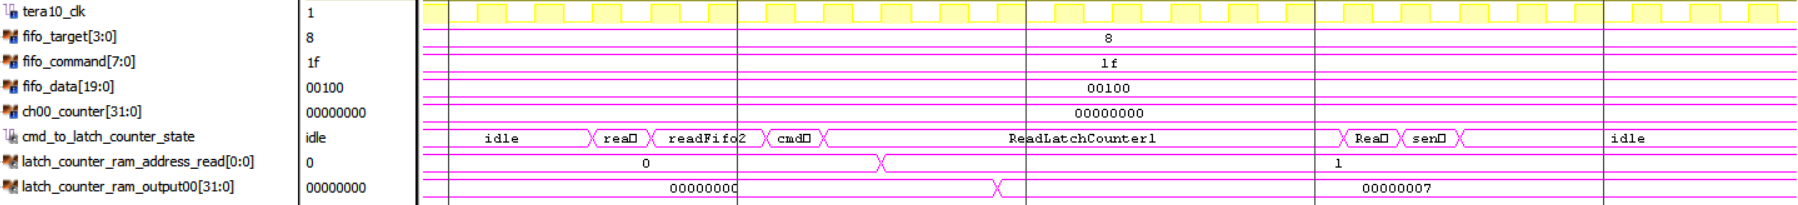
\includegraphics[width=1.0\linewidth]{IMG/ch4/LATCHsimulations/READLATCH}
	\caption{}
	\label{fig:readlatch}
\end{figure}
\noindent The next step is to send the correct 32~bit RAM output signal to the GbPhy module and thus to the computer.
The 192 individually implemented RAM components are divided into the four main categories introduced before (hit counters, clock counters, coincidence hit counters and coincidence clock counters).
The outputs of the RAMs of each main module are all connected to a 8~bit multiplexer. Each multiplexer is controlled by the fifo\_data(7 downto 0). These four multiplexers are then connected to another 4-inputs 1-output MUX controlled by the fifo\_command (sub-system command id). In this way the user can obtain and read only the desired signal.
In figure \ref{fig:replylatch} it can be seen a simulation of the of the reply from a read latch counter command.
The first signal is the 125~MHz clock, followed by the received packet, the FSM state and the RAM output signal.
The next signal, \textit{read\_latch\_counter\_reply[15:0]} is the 16~bit output from the first main MUX which is updated after one clock stroke of the RAM output.
This signal is then concatenated with the sub-system target (4~bit), the sub-system command ID (8~bit) and 4 padding zeros into a 32~bit reply string (\textit{command\_reply\_contents[31:0]}) that is sent to the PC. 
\begin{figure}[H]
	\centering
	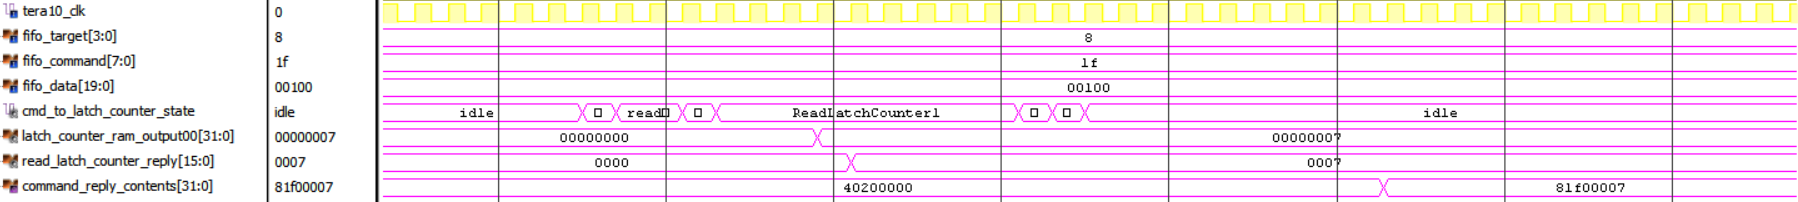
\includegraphics[width=1.0\linewidth]{IMG/ch4/LATCHsimulations/REPLYLATCH}
	\caption{}
	\label{fig:replylatch}
\end{figure}
\subsubsection{Implementation}
When coding HDL it is extremely important to always remember that every line of the code correspond to a real physical object inside the FPGA die. This means that if the user is adding FIFOs, BRAMs or LUTs the Vivado software suite needs create a new place every new component in such a way that the timing requirements are still met.
It is thus interesting to observe how the placement changes when new features are added to the firmware.
Figures \ref{fig:counters_clocks} and \ref{fig:allcounters} show the post-routing device view for two different moments of the latch counter module development. The figure on the left refers to a firmware version with only 96 latched counters while on the right all 192 RAM modules are implemented and working.
The two most important modules to observe in this pictures are: \textit{tera10\_latch\_counter} in yellow and \textit{tera10\_io} in green.
The Block RAMs are placed inside the die in strips and in the device representation are coloured in red; in total it can be observed 7 red RAM strips that corresponds to a total of 445 blocks.
In figure \ref{fig:counters_clocks} the number of used RAM blocks is low, thus the placer decided to group together the I/O logic (green).
In figure \ref{fig:allcounters} the number of used RAM blocks doubled, and it is not efficient to group together all the cell from the I/O module. The placer decided to spread-out the design and placed the counting logic in the nearest position to the respective RAM component. In this way when a \textit{do\_latch} signal is provided the path between the counter and the RAM input is always the lowest possible. 
\begin{figure}[H]
	\centering
	\begin{minipage}{.5\textwidth}
		\centering
		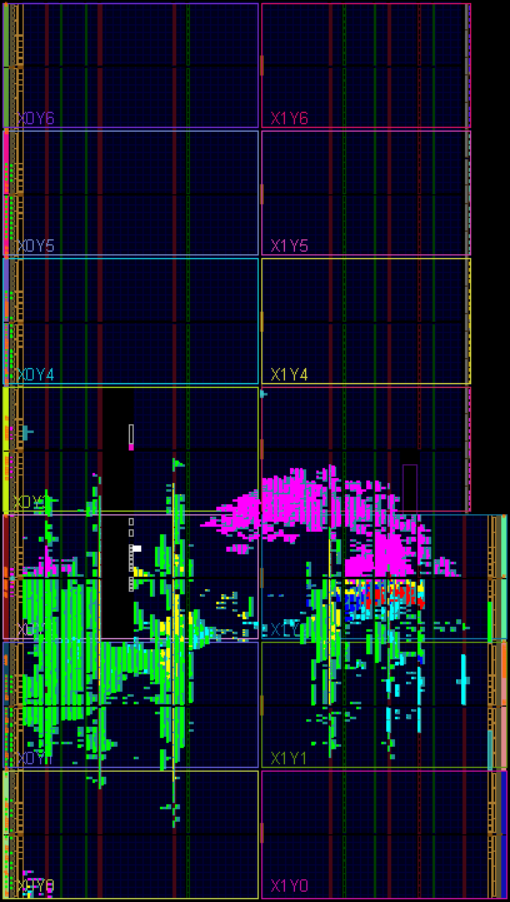
\includegraphics[width=.85\linewidth]{IMG/ch4/routed_colored_counters_clocks}
		\caption{Post-routing device view\\ with 96 counters latched.}
		\label{fig:counters_clocks}
	\end{minipage}%
	\begin{minipage}{.5\textwidth}
		\centering
		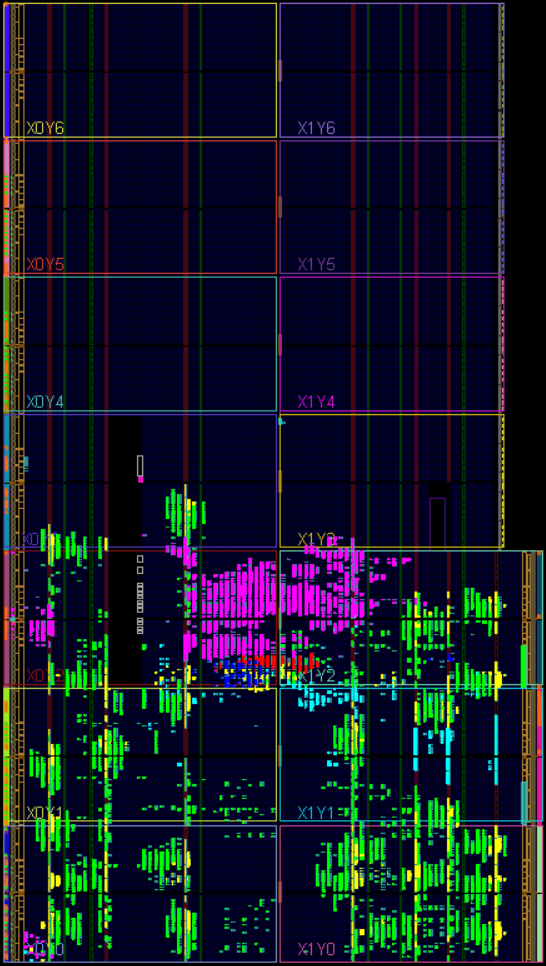
\includegraphics[width=.85\linewidth]{IMG/ch4/routed_colored_perfect}
		\caption{Post-routing device view\\ with all 192 counters latched.}
		\label{fig:allcounters}
	\end{minipage}
\end{figure}
\subsubsection{Timing}
\noindent The Vivado design suite has a Design Timing Report Summary that allows the user to easily rate the timing behaviour of the design.
An example of a report from this tool is depicted in figure \ref{fig:timingperfect}.
The Worst Negative Slack (WNS) is the slack value, in nano-seconds (ns), of the path with the worst timing. In this case this value is 0.122~ns which is greater than zero. This means that the path with the worst timing still meets the constraints.
The Total Negative Slack (TNS) is the slack sum of every path that do not met timing constraints. In this case it is 0,000~ns; this means that there are NO problematic paths in the implemented design.

\begin{figure}[H]
	\centering
	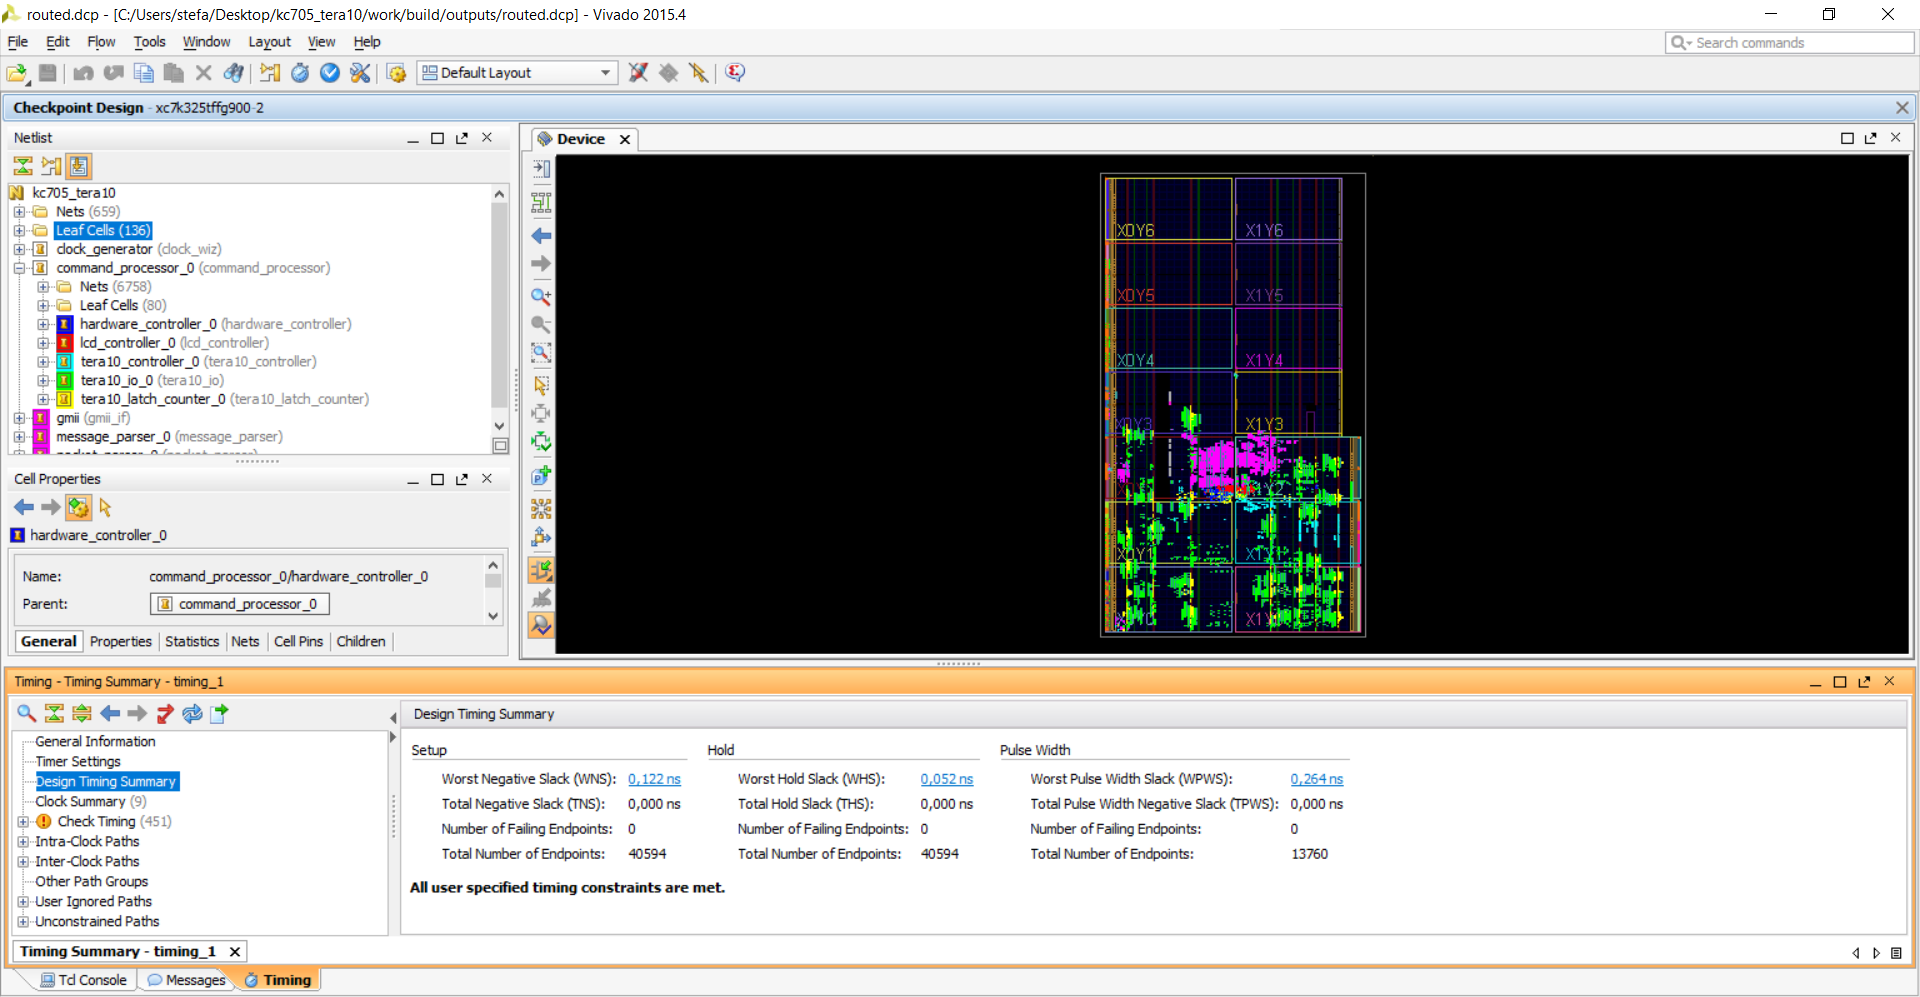
\includegraphics[width=0.95\linewidth]{IMG/ch4/TIMING_perfect}
	\caption{Design Timing Report Summary for kc705\_tera10 firmware; All user specified timing constraints are met.}
	\label{fig:timingperfect}
\end{figure}

\subsection{Timestamp generator}\label{Timestamp}
\noindent The previous section described how the current state of every counter was saved into a RAM.
This latch mechanism allows to synchronize the measurement of counts from different channel.
In order to calculate the count rate, it is needed to compare two measurements of counts with the time elapsed between two latches.
This time is provided by a timestamp generated in correspondence to each latch and saved into a register.
The hearth of a time measuring device is a event generator with well defined period, thus a clock signal.
The first process implemented is a 500~MHz (2~ns period) counter.
Using a 64~bit register means that the maximum time interval measurable is:
\begin{equation}
	2 \: ns \cdot \: 64 \: bit \: =\: 2 \: ns \cdot \: 18.44\cdot10^{18} \: = \: 36.6\cdot10^{9} \: s \approx 1170 \: years 
\end{equation}
\noindent With a 64 bit counter the FPGA could stay ON for more than 1000 years and still count without resetting the register. 1170 years is overkill, however the Xilinx Kintex 7 has many more resources than the project needs, thus the use of a 64 bit counter is acceptable.
The counting process runs on a 500~MHz clock (the same clock used for the de-serializer) while the \textit{tera10\_latch\_counter} module runs on a 125~MHz clock. In order to enable the data flow between the two domain, without causing time violation errors, I used a (Clock Domain Crossing) CDC-FIFO memory IP, as shown in figure \ref{fig:fifo_ip}.
This automatically generated module has a 64~bit write width, a depth of 512 (the minimum for this type of Built/in FIFO), six inputs and three outputs:
\begin{itemize}
	\item \textit{rst}: reset signal; active \textit{high};
	\item \textit{wr\_clk}: write clock; 500~MHz clock used for the timestamp counter;
	\item \textit{rd\_clk}: read clock; 125~MHz clock used for the \textit{tera\_latch\_counter} processes;
	\item \textit{din[63:0]}: data in; 64~bit input signal at 500~MHz;
	\item \textit{wr\_en}: write enable; when the signal is \textit{high} the logic transfers the \textit{din} signal into the memory;
	\item \textit{rd\_en}: read enable; when the signal is \textit{high} the logic transfers the data from the memory to the \textit{dout} signal;
	\item \textit{full}: output signal, when the FIFO memory if full this signal is \textit{high};
	\item \textit{empty}: output signal, when the FIFO memory is empty this signal is \textit{high};
	\item \textit{dout[63:0]}: data out; 64~bit output signal at 125~MHz;
\end{itemize}
\begin{figure}[H]
	\centering
	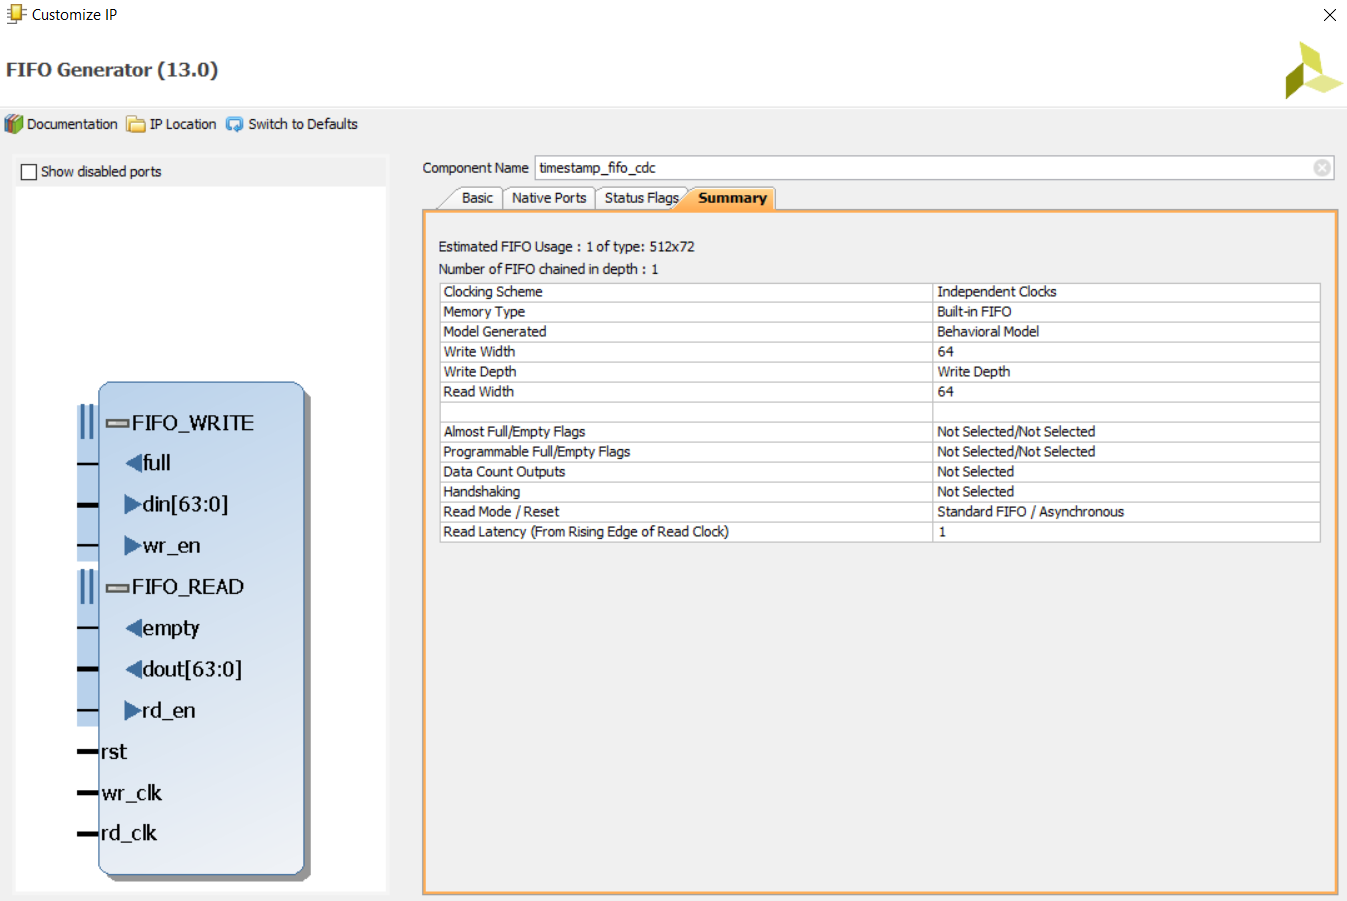
\includegraphics[width=0.6\linewidth]{IMG/ch4/FIFO_IP}
	\caption{Vivado IP manager summary for CDC FIFO Memory IP}
	\label{fig:fifo_ip}
\end{figure}
\noindent I then added two sub-system commands IDs to the ones described in section \ref{Latch}:
\begin{itemize}
	\item \textit{0x5F} => \textit{do timestamp}:
	\begin{itemize}
		\item fifo\_data(11 downto 8) = read address (from \textit{0x0} to \textit{0xF})
		\item fifo\_data(7 downto 0) = don't care
	\end{itemize}
	\item \textit{0x6F} => \textit{read timestamp}:
	\begin{itemize}
		\item fifo\_data(11 downto 8) = read address (from \textit{0x0} to \textit{0xF})
		\item fifo\_data(7 downto 0) = select data portion (from \textit{0x00} to \textit{0x03})
		\begin{itemize}
			\item "\textit{0000\_0000}" = fifo\_reply(15 downto 0) <= timestamp(15 downto 0)
			\item "\textit{0000\_0001}" = fifo\_reply(15 downto 0) <= timestamp(31 downto 16)
			\item "\textit{0000\_0010}" = fifo\_reply(15 downto 0) <= timestamp(47 downto 32)
			\item "\textit{0000\_0011}" = fifo\_reply(15 downto 0) <= timestamp(63 downto 48)
		\end{itemize}
	\end{itemize}
\end{itemize}
\noindent It has to be noted that when a \textit{do\_latch} command is performed also the \textit{do\_timestamp} process is activated.
The \textit{do\_timestamp} signal runs on the 125~MHz clock and has a duration of several 500~MHz clock strokes. The logic that latches the counter and uses this signal as a trigger runs on this second, faster, clock.
This means that the trigger signal is being oversampled and thus no timing violation is being created.
However, if the logic receives the \textit{do\_timestamp} signal for multiple clock cycles it could overwrite the timestamp and thus ruin the data.
In order to prevent that I implemented an extremely simple FSM, shown in figure \ref{fig:timestampFSM}, that ensures that the timestamp counter is being latched only once for each trigger signal.
\begin{figure}[H]
	\centering
	\includegraphics[width=0.85\linewidth]{FSMdiagrams/timestampFSM.pdf}
	\caption{Timestamp latch FSM diagram.}
	\label{fig:timestampFSM}
\end{figure}
\noindent Figure \ref{fig:timestampfsm} shows the result of a simulation of the FSM behaviour.
The first signal is the 500~MHz clock followed in the next row by the values of the 64~bit counter updated each rising edge clock. The third signal is the \textit{do\_timestamp} trigger. The fourth is the FSM state.
From the \textit{idle} state when \textit{do\_timestamp} is \textit{high} it goes to \textit{dotimestamp1}. In this state the latching is done and the data is temporally saved into a register (\textit{timestamp\_signal[63:0]}). At the next rising edge of the clock it switches to \textit{dotimestamp2} (WAIT in figure \ref{fig:timestampFSM}) and sits here until \textit{do\_timestamp} turns \textit{low}. Then it goes back to IDLE ready for another trigger.
\begin{figure}[H]
	\centering
	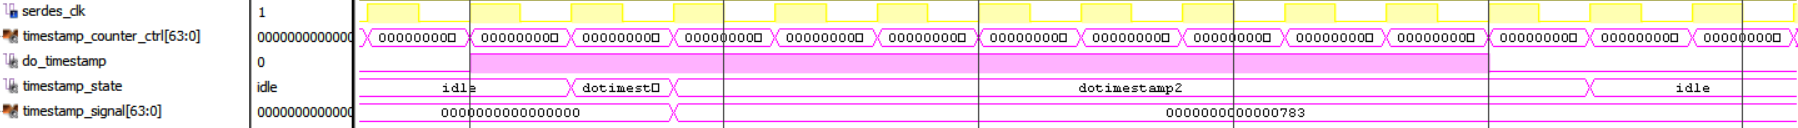
\includegraphics[width=1.0\linewidth]{IMG/ch4/TIMESTAMPsimulations/TIMESTAMPFSM}
	\caption{}
	\label{fig:timestampfsm}
\end{figure}
\noindent The \textit{timestamp\_signal[63:0]} signal needs to cross from one clock domain to another.
For this purpose the CDC-FIFO is used.
In figure \ref{fig:timestampfifo} it can be seen a simulation of this memory component. 
The first two signals are the write clock (500~MHz) and the read clock (125~MHz).
While the FSM is in the \textit{dotimestamp2} state the write enable signal (\textit{wr\_en}) turns \textit{high}.
This means that, right before enabling the writing into the FIFO at the input, the correct signal appears (\textit{din[63:0]}). 
This design is based on the assumption that only one timestamp at the time is generated, thus the memory either is empty or it contains only one data.
If the memory is not empty the signal \textit{empty} goes \textit{low} and at the next rising edge of the read clock the read enable (\textit{rd\_en}) signal goes \textit{high}.
When the read enable signal is \textit{high} the timestamp data appears at the output FIFO memory (\textit{dout[63:0]}) and at the same time the \textit{timestamp\_ram\_write\_en} signal goes to '\textit{1}'.
This allows the data to be stored into a 64~bit width 16 depth RAM memory as explained in the previous section; ready to be read and sent to the PC.
\begin{figure}[H]
	\centering
	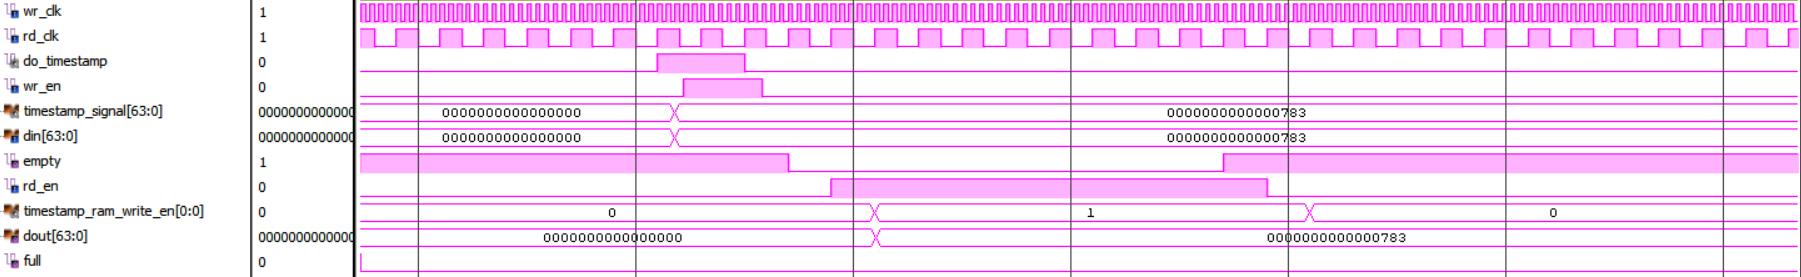
\includegraphics[width=1.0\linewidth]{IMG/ch4/TIMESTAMPsimulations/TIMESTAMPFIFO}
	\caption{}
	\label{fig:timestampfifo}
\end{figure}
\noindent In order to read the entire 64~bit signal the data are divided into four 16~bit pieces. Each part of the timestamp (0 down to 15; 16 down to 31; 32 down to 47; 48 down to 63) have to be individually read with a command and then reassembled in software. 

\subsubsection{Implementation}
\noindent It is interesting to observe how the placer managed this new addition to the firmware. The FIFO memory is implemented with a Built-in FIFO, this means that inside the FPGA die there is a portion of space built with the purpose to be a FIFO. This makes the IP extremely efficient and less space hungry.
In this design the FIFO is only used to cross the clock domain, it stores at maximum one 64~bit array. The data is stored into a RAM in order to allow random writes and reads.
In figure \ref{fig:fifonearram} it can be seen that the placer "decided" to place the RAM Block (in green) in the nearest possible position to the FIFO Block (in red) in order to minimize the path delay.
The yellow blocks are the location of the logic cells of the \textit{tera10\_latch\_counter} module used to control the FIFO and the RAM.
\begin{figure}[H]
	\centering
	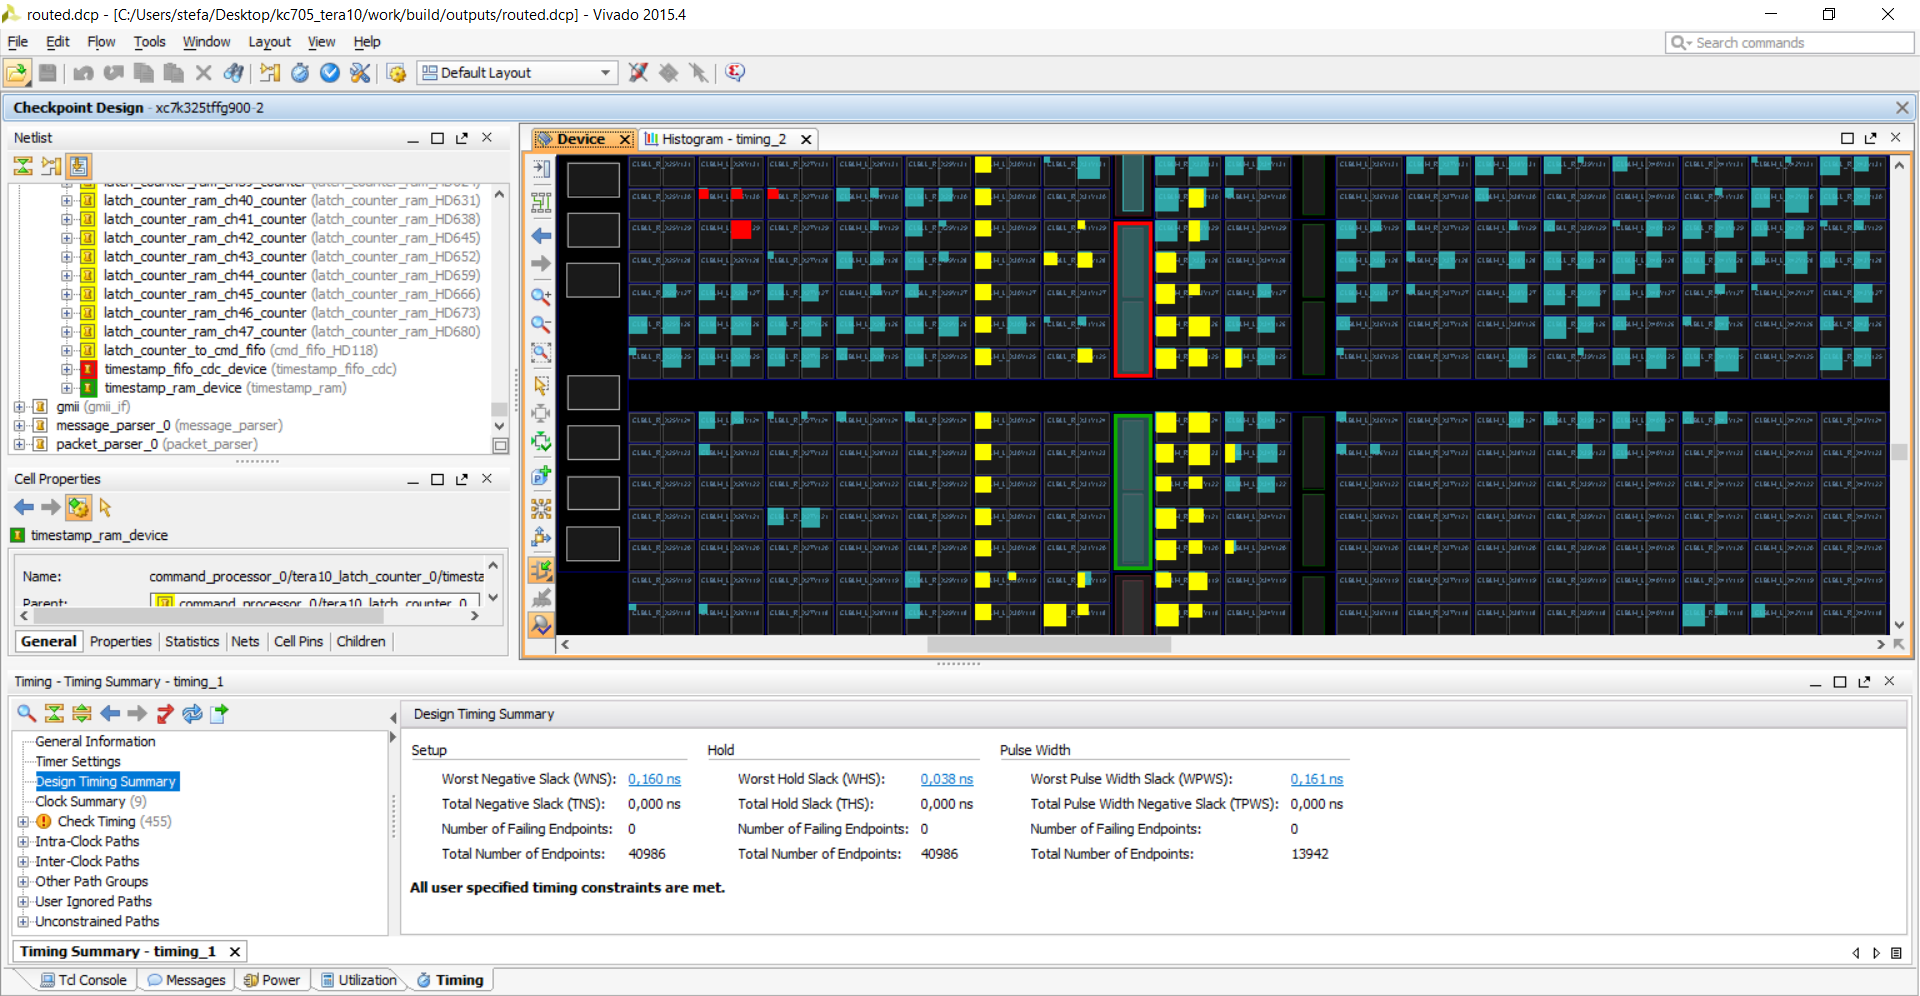
\includegraphics[width=0.95\linewidth]{IMG/ch4/FIFOnearRAM}
	\caption{Device view with focus on timestamp FIFO and RAM placement.}
	\label{fig:fifonearram}
\end{figure}

\section{Final firmware reports}
In this section the output results from the implementation of the final firmware version are analyzed.
This last implementation was done with two different configurations, in order to understand the differences between them.
Usually a HDL design has a top entity and in the top architecture some components are instantiated and in those components architectures some other modules can be instantiated. This is called design hierarchy. Each component has its own input/output ports used to interface with its parents entity and its child components. Those ports form the "hierarchy" boundaries. A hierarchy diagram can be seen in figure \ref{fig:tera10}.
During the implementation process the \textit{flatten\_hierarchy} option controls how the Synthesis tool handles those hierarchy boundaries.
"Full" means to break those boundaries and have a flattened netlist. Thus, all elements are in the same hierarchy. "None" means keeping all boundaries as they are described in the RTL.
In this section the differences between these two results are analyzed. In figure \ref{fig:noflatdevice} the logic has not been flattened while in figure \ref{fig:flatdevice} the logic was flattened. It can be seen an important difference in the placement layout, however a RAM block is still a RAM block and has to be placed in more or less the same spot.

\begin{figure}[H]
	\centering
	\begin{minipage}{.5\textwidth}
		\centering
		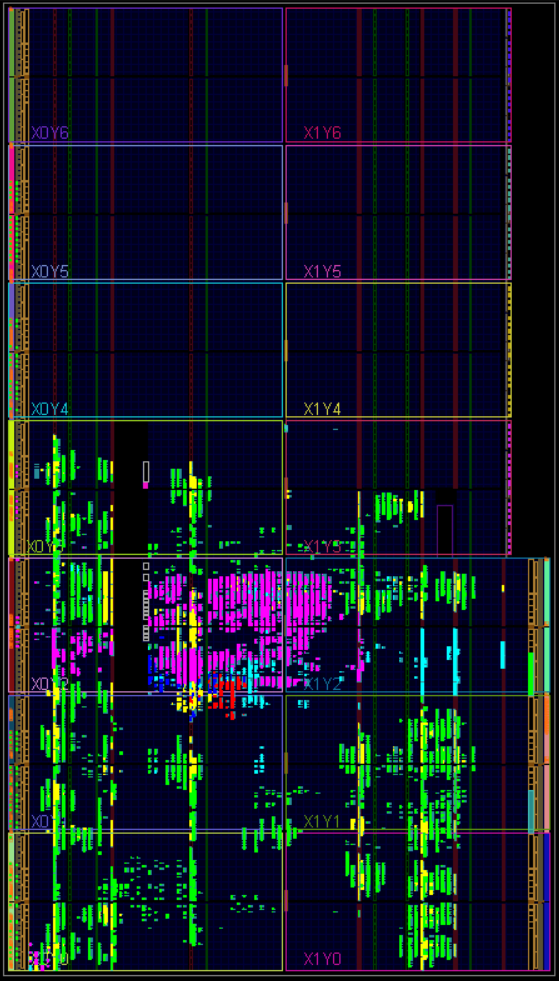
\includegraphics[width=.85\linewidth]{IMG/ch4/FirmwareNOFLAT/DEVICE}
		\caption{Firmware device view \\with NON flattened logic.}
		\label{fig:noflatdevice}
	\end{minipage}%
	\begin{minipage}{.5\textwidth}
		\centering
		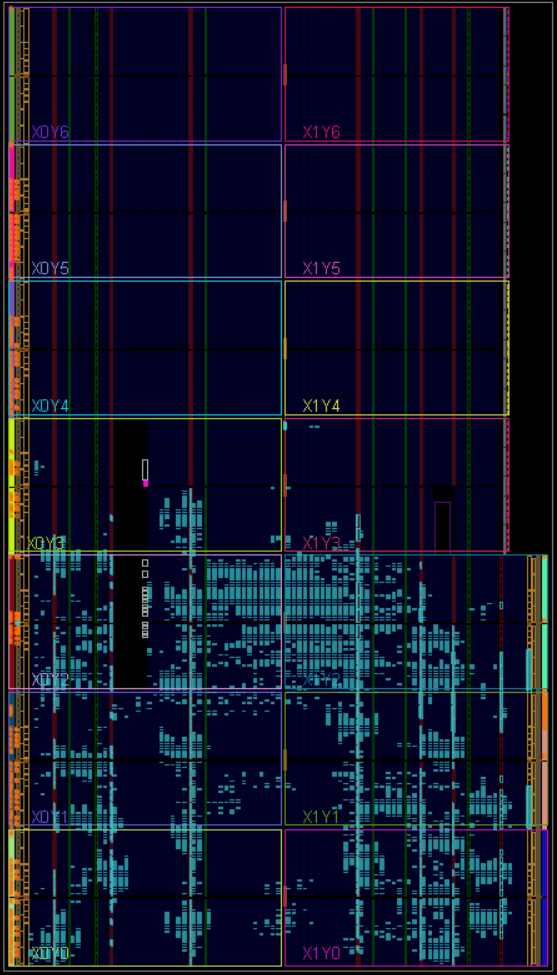
\includegraphics[width=.85\linewidth]{IMG/ch4/FirmwareFLAT/DEVICE}
		\caption{Firmware device view \\with flattened logic.}
		\label{fig:flatdevice}
	\end{minipage}
\end{figure}
\noindent It is worth noting that with a flat hierarchy the division between modules with different colours can not be done. In fact there are no modules and components, the logic is all at the same "level".
For both of these implementations three type of reports have been performed: TIMING, POWER and UTILIZATION.

\subsubsection{Final timing report}
\noindent In figures \ref{fig:noflattiming} and \ref{fig:flattiming} it can be seen that in both cases the timing requirements are met, the number of total endpoints is the same (40986). The values of Worst Negative Slack (WNS) and Worst Hold Slack (WHS) are slightly different, but not by much. It should be considered that for our purpose any value greater than zero is acceptable.
A small difference in WNS (if still positive) will not affect the operation of the device.  
\begin{figure}[H]
	\centering
	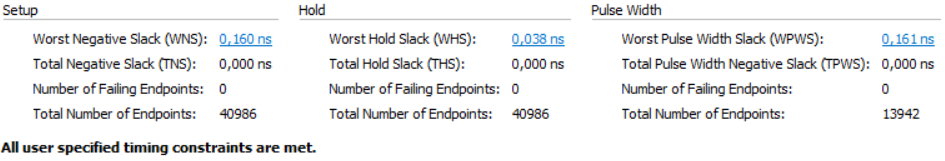
\includegraphics[width=0.8\linewidth]{IMG/ch4/FirmwareNOFLAT/TIMING}
	\caption{Timing report with hierarchical logic.}
	\label{fig:noflattiming}
\end{figure}

\begin{figure}[H]
	\centering
	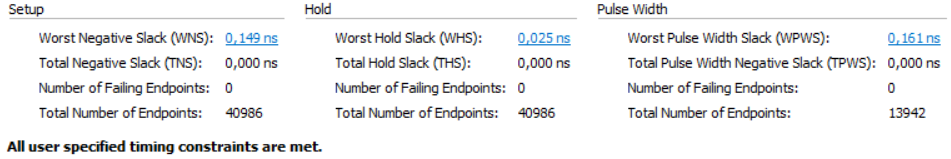
\includegraphics[width=0.8\linewidth]{IMG/ch4/FirmwareFLAT/TIMING}
	\caption{Timing report with flattened logic.}
	\label{fig:flattiming}
\end{figure}

\subsubsection{Final power report}
\noindent Figures \ref{fig:noflatpower} and \ref{fig:flatpower} show the on-chip power report for each case.
The reported value of 1.825~W is an estimation of the dynamic power consumption of the logic alone, not of the entire board, that has to deliver power to many more component, such as LCD display and backlight, LEDs, cooling fan, I/O pins, voltage converters, JTAG and PHY daughter boards and more.
It is interesting to consider how the power consumption is divided. Almost 40\% of the total energy drawn is due to the RAM memory, this means that my additions to the firmware had a measurable impact on the on-chip power. However this values are still extremely low and, in addition, this application has no tight power constraints.
Thus we can use this numbers only for our interest without being too much concerned about efficiency. 
\begin{figure}[H]
	\centering
	\begin{minipage}{.5\textwidth}
		\centering
		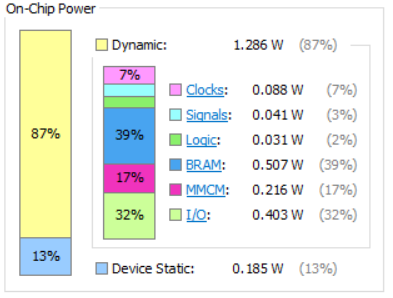
\includegraphics[width=.9\linewidth]{IMG/ch4/FirmwareNOFLAT/POWER}
		\caption{Power report with \\hierarchical logic.}
		\label{fig:noflatpower}
	\end{minipage}%
	\begin{minipage}{.5\textwidth}
		\centering
		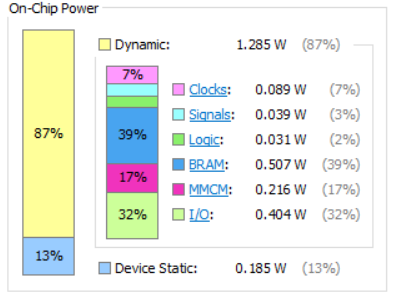
\includegraphics[width=.9\linewidth]{IMG/ch4/FirmwareFLAT/POWER}
		\caption{Power report with \\flattened logic.}
		\label{fig:flatpower}
	\end{minipage}
\end{figure}
\subsubsection{Final utilization report}\label{UtilizationReport}
\noindent In figures \ref{fig:noflatutilization} and \ref{fig:flatutilization} it can be seen the utilization report for each case. The two tables are almost identical, the only difference is that the flattened design uses three LUTs less. Not that big of a difference considering that the total available LUTs are 203800.
This means that this design is already well optimized and the flattening did not affected much the resources utilization.
The two more used resources are the BRAM, used for the implementation of the latch and the timestamp, and the I/O ports, used to communicated with the testboards and thus with the chips.
It should be noted that no FPGA primitive is used for more that 50\%. The KC705 board is extremely capable; More feature could be therefore added without any board limitation. 
\begin{figure}[H]
	\centering
	\begin{minipage}{.5\textwidth}
		\centering
		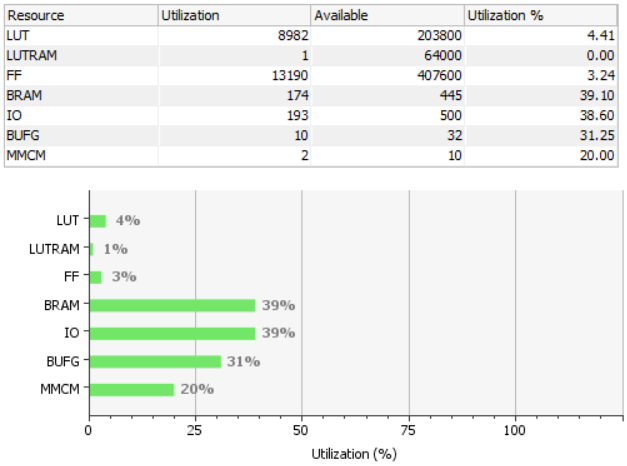
\includegraphics[width=.99\linewidth]{IMG/ch4/FirmwareNOFLAT/UTILIZATION}
		\caption{Utilization report with \\hierarchical logic.}
		\label{fig:noflatutilization}
	\end{minipage}%
	\begin{minipage}{.5\textwidth}
		\centering
		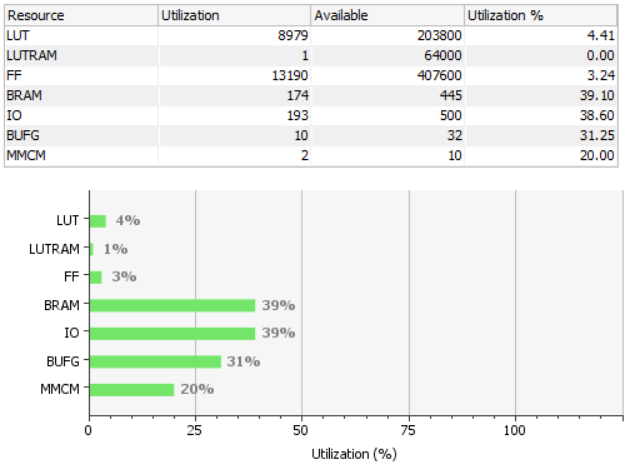
\includegraphics[width=.99\linewidth]{IMG/ch4/FirmwareFLAT/UTILIZATION}
		\caption{Utilization report with \\flattened logic.}
		\label{fig:flatutilization}
	\end{minipage}
\end{figure}
\noindent In this particular case the differences between flattened and non-flattened implementation is negligible. I opted for the non-flattened design.


